
\chapter{Benchmarking the Performance of the CMS Level-1 Trigger}
\label{subsec:l1trigger}

This chapter describes and details the work performed by the author, in measuring the performance of L1 single jet and energy sum triggers in the \acf{GCT} during the 2012-2013 run period. The \ac{CMS} \ac{GCT} is the device within the \L1 CMS calorimeter trigger system which is assigned the tasks of finding and sorting forward, central and $\tau$-jet candidates (hadronically decaying $\tau$'s), sorting isolated and non-isolated electron candidates and reading out all of the calorimeter trigger data. The \ac{GCT} system is installed in the \ac{CMS} underground cavern. 

The \L1 trigger is an extremely important component in the recording of proton-proton collisions by the \ac{CMS} detector. Good performance by the \L1 systems will ensure that the rate at which collisions are recorded remain at a manageable level whilst maintaining low trigger thresholds, which in turn increases sensitivity to a range of physics signatures. 

A change was introduced to the \L1 jet clustering algorithm (see Section (\ref{subsec:l1jettrigger})) half way through the 2012 run period. This change was made to reduce the number of jets clustered by the \L1 jet algorithm as a result of the isotropic deposits left in the \ac{CMS} calorimeters from multiple pile-up interactions. Such jets would result in a large increase in the trigger rate of both the individual \L1 jet and combined transverse energy scale sum, \theht, triggers. 

Jets that result from pile-up typically have a diffuse spread of energy across the whole area of the jet in comparison to central energy deposits in jets arising from the primary interaction. Therefore a 5 \GeV central seed threshold was introduced to prevent the formation of these pile-up jets. 

The effect of this change on the performance of the \L1 trigger is benchmarked in Section (\ref{subsec:l1jetseedpu}). The two run periods that are used in this chapter to compare trigger performance before and after the introduction of a central jet seed threshold are known as Run 2012B and Run 2012C respectively. They reflect the period prior and after the extended shutdown period of the \ac{lhc} when this change was implemented. 

 Additionally the \L1 \ac{GCT} performance is also measured as a function of different pile-up (first introduced in Section (\ref{sec:thelhc})) conditions which occurred during the Run 2012C period in Section (\ref{subsec:l1jetpu}).

\section{The Level-1 Trigger}

\label{sec:l1trigger}

The \L1 trigger reduces the rate of events collected from 20 MHz to approximately 100 kHz using information from just the calorimeters and muon chambers, but not the tracker. This is due to requirement that data from each and every bunch crossing be analysed with no dead time, drastically reducing time available to process and reconstruct objects in making a trigger decision. This facilitates the need for a pipelined processing architecture, and so a tree system of triggers is used to decide whether to pass on an event to the \ac{HLT} for further reconstruction.

Calorimeter and muon event information is processed separately by the \acf{RCT} and \acf{RMT} systems respectively and which are located within the \ac{CMS} cavern. Within the \ac{RCT}, energy deposits from trigger towers in the \ac{ECAL} and \ac{HCAL} calorimeters are summed into coarser calorimeter regions and sent to the \acf{GCT} for jet clustering.

Given that electron, $e$, and photon, $\gamma$, are much narrower objects than jets, the \ac{RCT} is used to identify these candidates but makes no attempt to distinguish between them at this stage given the lack of tracking information. They are first identified by ensuring the energy deposits within the central trigger tower and its surrounding cells are above a certain programmable threshold. To ensure the object is not a hadron, the ratio of \ac{HCAL} to \ac{ECAL} in the central tower is calculated and checked to be below 5\%. Additional algorithms are employed to ascertain whether the e/$\gamma$ object is isolated/non-isolated.

In the \L1 \ac{GCT}, coarse measurements of the energy deposited in the electromagnetic and hadronic calorimeters are combined, and by using sophisticated algorithms the following tasks are performed:

\begin{itemize}
	\item isolated and non-isolated electromagnetic objects are sorted (e and $\gamma$), with the four highest ranked (equivalent to highest transverse energy $E_{T}$) objects of each type passed onto the \ac{GT} which with the addition of information from the muon systems makes the final trigger pass/fail decision,
	\item energy sums from the calorimeters supplied by the \ac{RCT} are used in performing jet clustering (described in the following section). The clustered jets are then sub-divided into categories depending on their pseudo-rapidity and the result of $\tau$ identi�cation, being classified as either central, forward, or tau ($\tau$). After being sorted by decreasing energy, the four highest of each category are passed to the \ac{GT} for use in trigger decisions,
	\item total transverse energy ($\et = \sum_{i=1}^{n} E_{T}^{obj_{i}}$), the scalar sum of the energy deposits measured by L1,  and missing transverse energy ($\met = \lvert \sum_{i=1}^{n} E_{T}^{obj_{i}} \rvert$), defined as the negative vector sum of the transverse energy deposits measured at \L1 are calculated,
	\item total transverse jet energy ($\theht = \sum_{i=1}^{n} E_{T}^{jet_{i}}$), the scalar sum of the energy of all L1 clustered jet objects, and missing transverse jet energy ($\mht =  \lvert \sum_{i=1}^{n} E_{T}^{jet_{i}} \rvert$), defined as the negative vector sum of the energy from L1 clustered jet objects are calculated and passed to the \ac{GT}. 
\end{itemize}

In addition, quantities suitable for triggering minimum bias events, forward physics and beam background events are determined. Relevant muon isolation information is also passed on to the \acf{GMT} to be used in decisions involving the muon triggers, where it is combined with information from across the three muon sub-systems. The resultant final accept/reject decision at \ac{L1} is then performed by the \ac{GT}, based on the objects received from the \ac{GCT} and \ac{GMT} ($e/\gamma$, $\mu$, jets, $\et$, $\met$, $\theht$, $\mht$).

The \L1 trigger is therefore of upmost importance to the functioning of the detector. Without a high-performing, efficient trigger and a good understanding of its performance at ever increasing instantaneous luminosities, the data collected would be useless. Whilst it would be possible to maintain trigger efficiency by increasing the triggering thresholds for different jet or energy sum quantities, this is far from ideal. This could result in the failure to be sensitive to a wide range of new physics signatures, including many types of compressed spectra \ac{SUSY} models where the mass splitting between squarks/gluinos and the \ac{LSP} is small. 

\subsection{The \L1 Jet Trigger Algorithm}
\label{subsec:l1jettrigger}

The \L1 jet algorithm clusters jets using the transverse energy sums computed by the calorimeter trigger regions. Each region consists of  a $4 \times 4 $ trigger tower window which within the \ac{CMS} barrel spans a region of $\Delta \eta \times \Delta \phi = 0.087 \times 0.087$ in pseudorapidity-azimuth. 

A \L1 jet is defined by a $3 \times 3$ window of calorimeter regions, as shown in Figure \ref{fig:l1jetalgo}. This corresponds to $12 \times 12$ trigger towers in barrel and endcap. The $\phi$ size of the jet window is the same everywhere, whilst the $\eta$ binning increases at high $\eta$ due to calorimeter and trigger tower segmentation. The jets are labelled by the $(\eta, \phi)$ indices of the central calorimeter region.   

\begin{figure}[ht!]
\centering
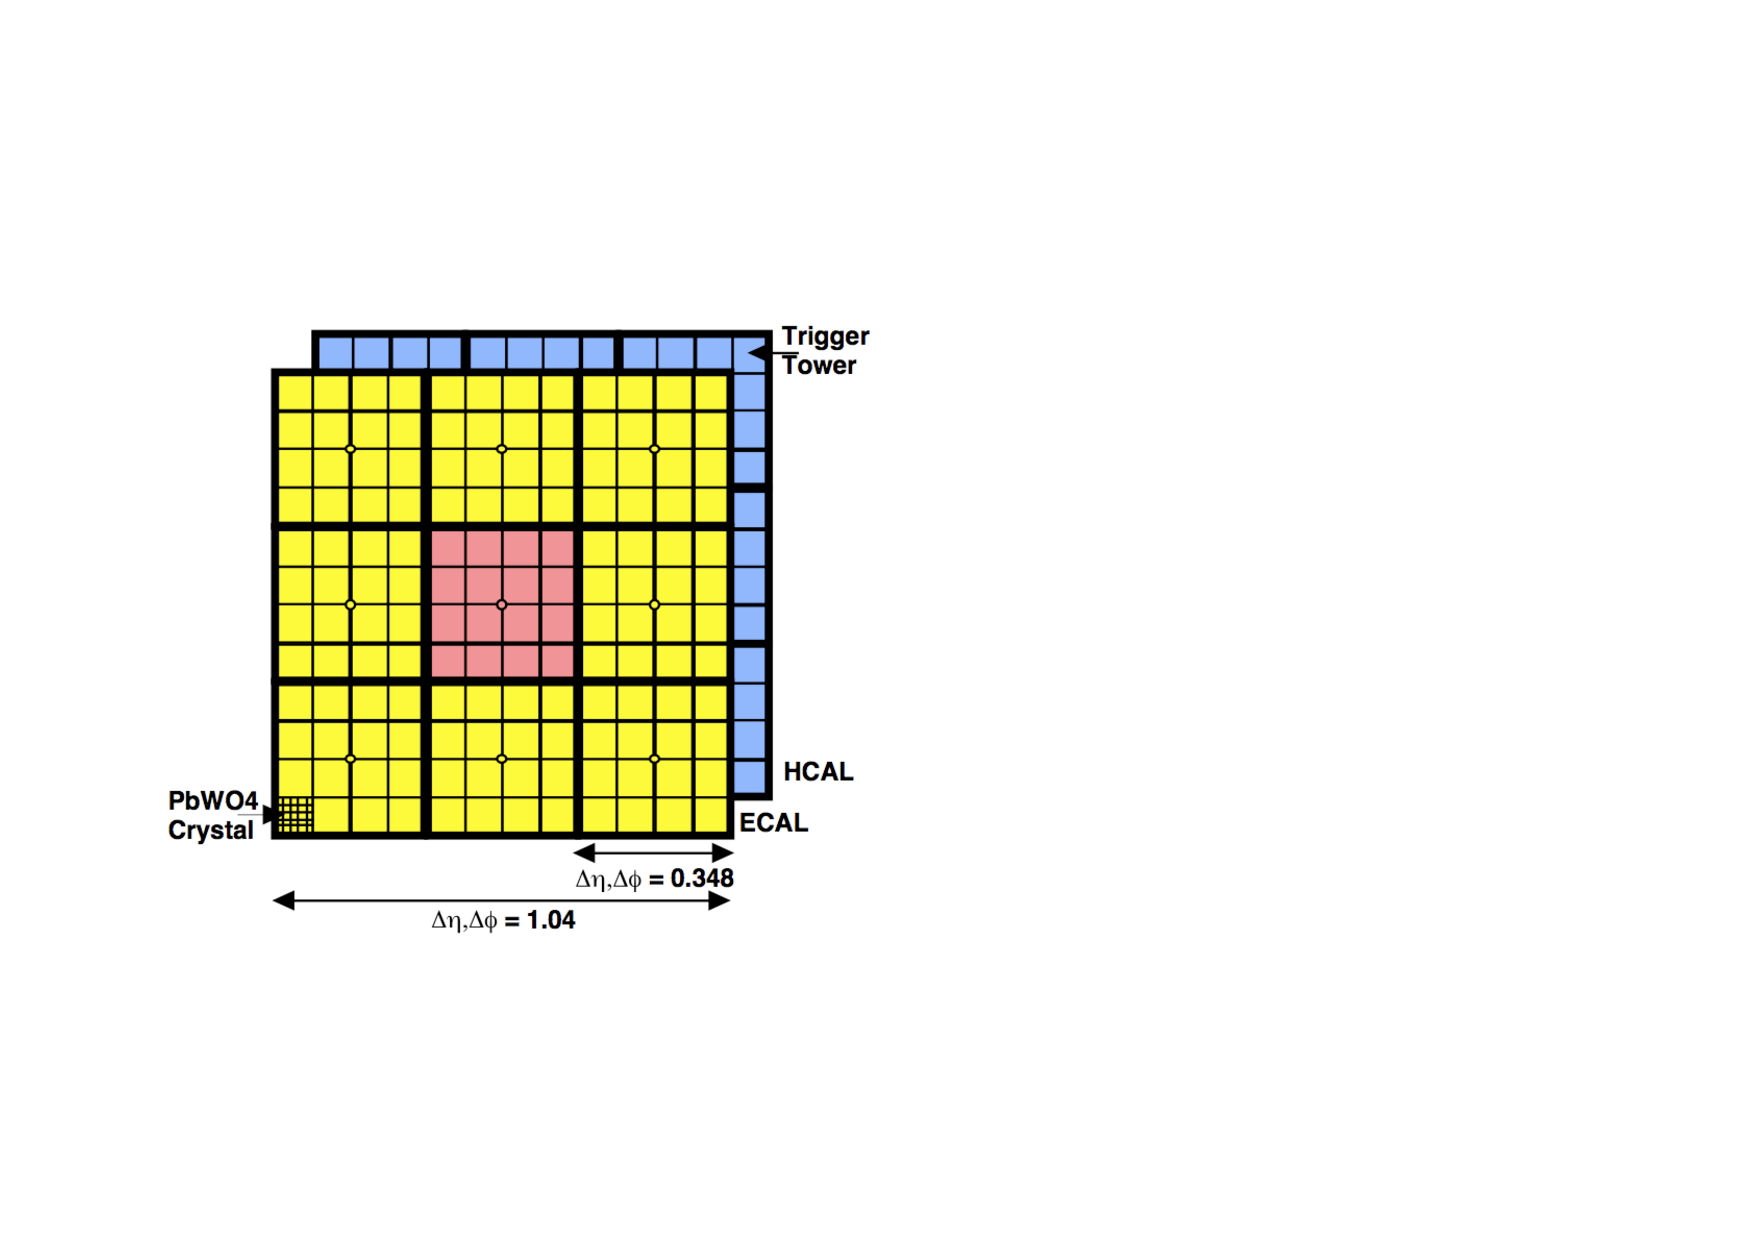
\includegraphics[width=0.55\textwidth]{plots/L1JetAlgorithm_v2.pdf}
\caption[Illustration of the dimensions of the Level-1 jet finder window.]{Illustration of the dimensions of the Level-1 jet finder window. Each cell represents a trigger tower, which is the sum of the transverse energy contributions from both calorimeter systems.}  
\label{fig:l1jetalgo}
\end{figure}  


A jet candidate is identified if the sum of the transverse \ac{ECAL} and \ac{HCAL} energies of a calorimeter region is larger than all of its eight neighbouring regions $E_{\text{T central}} > E_{\text{T surround}}$. This central region becomes the seed of the \L1 jet. 

During the 2012 run period, a minimum threshold of 5 \GeV was imposed on the central seeding region to suppress noise from non-collimated pile-up jets. This threshold is applied on the raw energy values deposited in the central calorimeter region and affects all clustered \L1 jets. The effect of such a change to the jet algorithm on the triggering performance of L1 quantities is shown in Section (\ref{subsec:l1jetseedpu}).

To form the jet candidates, the \ac{GCT} utilises a pre-clustering algorithm which employs 18 jet-finders operating in parallel over the whole detector. Each jet-finder spans an area of 11 calorimeter regions in $\eta$ (half the detector) and two in $\phi$ (40$\degree$).  

A depiction of how the clustering algorithm creates \L1 jets is shown in Figure \ref{fig:l1_stage}. Jets are initially created in $2\times 3$ mini-clusters within each jet finder in order to reduce the total amount of data duplicated and shared between the jet-finders (stage 1). Information is only shared with the two $\phi$ strips of the neighbouring jet-finders when these mini-clusters jets are found. If two mini-clusters in neighbouring strips are found adjacent to each other, the larger mini-cluster is kept (stage 2). A clustered $3 \times 3$ \L1 jet object is then formed from combining the $2\times 3$ mini-cluster with the $1\times 3$ window of trigger towers of the neighbouring strip (stage 3). \L1 jets are then sorted and passed onto the \ac{GT} for trigger decisions (stage 4).  

\begin{figure}[ht]
\centering
\begin{minipage}[b]{0.46 \linewidth}
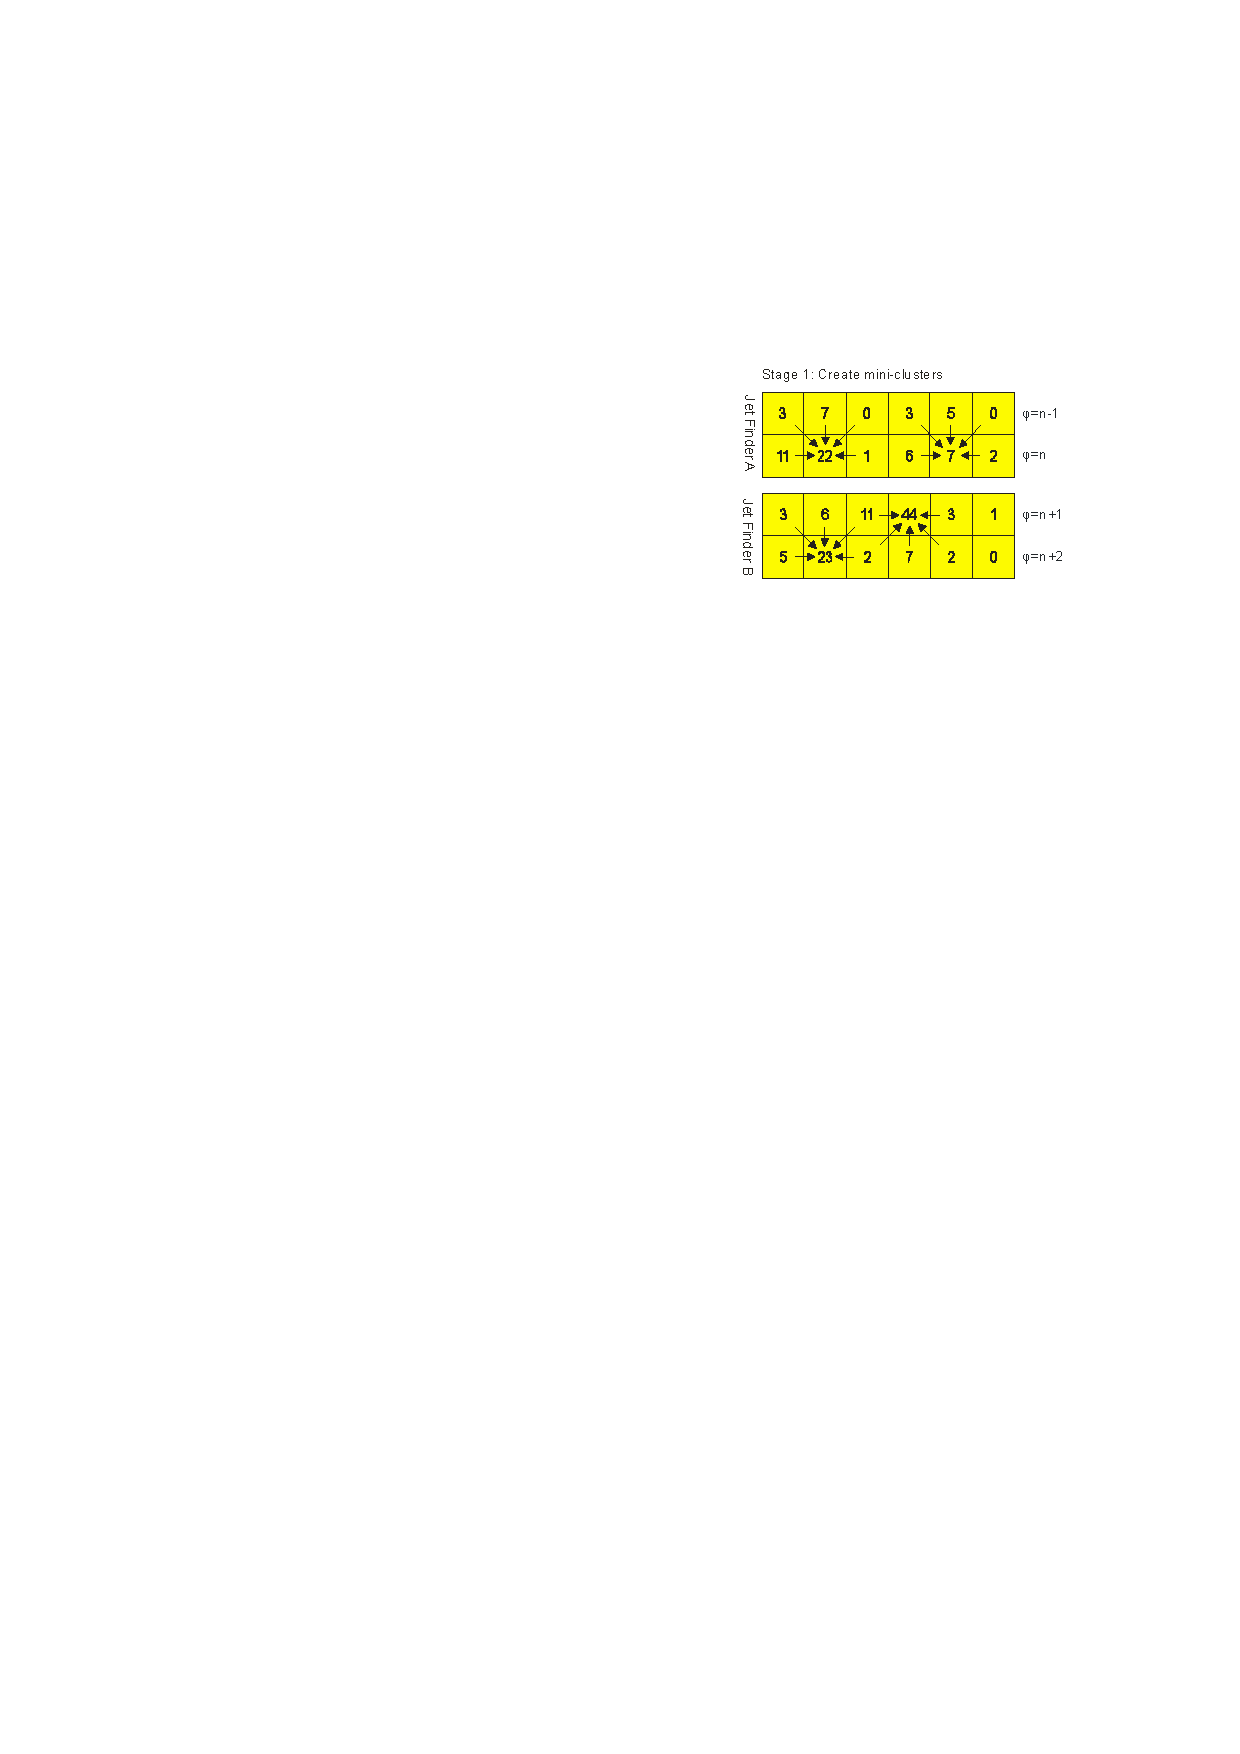
\includegraphics[width = 1.0\linewidth]{plots/l1trigger_stage1.pdf}
\end{minipage}
\quad
\begin{minipage}[b]{0.46 \linewidth}
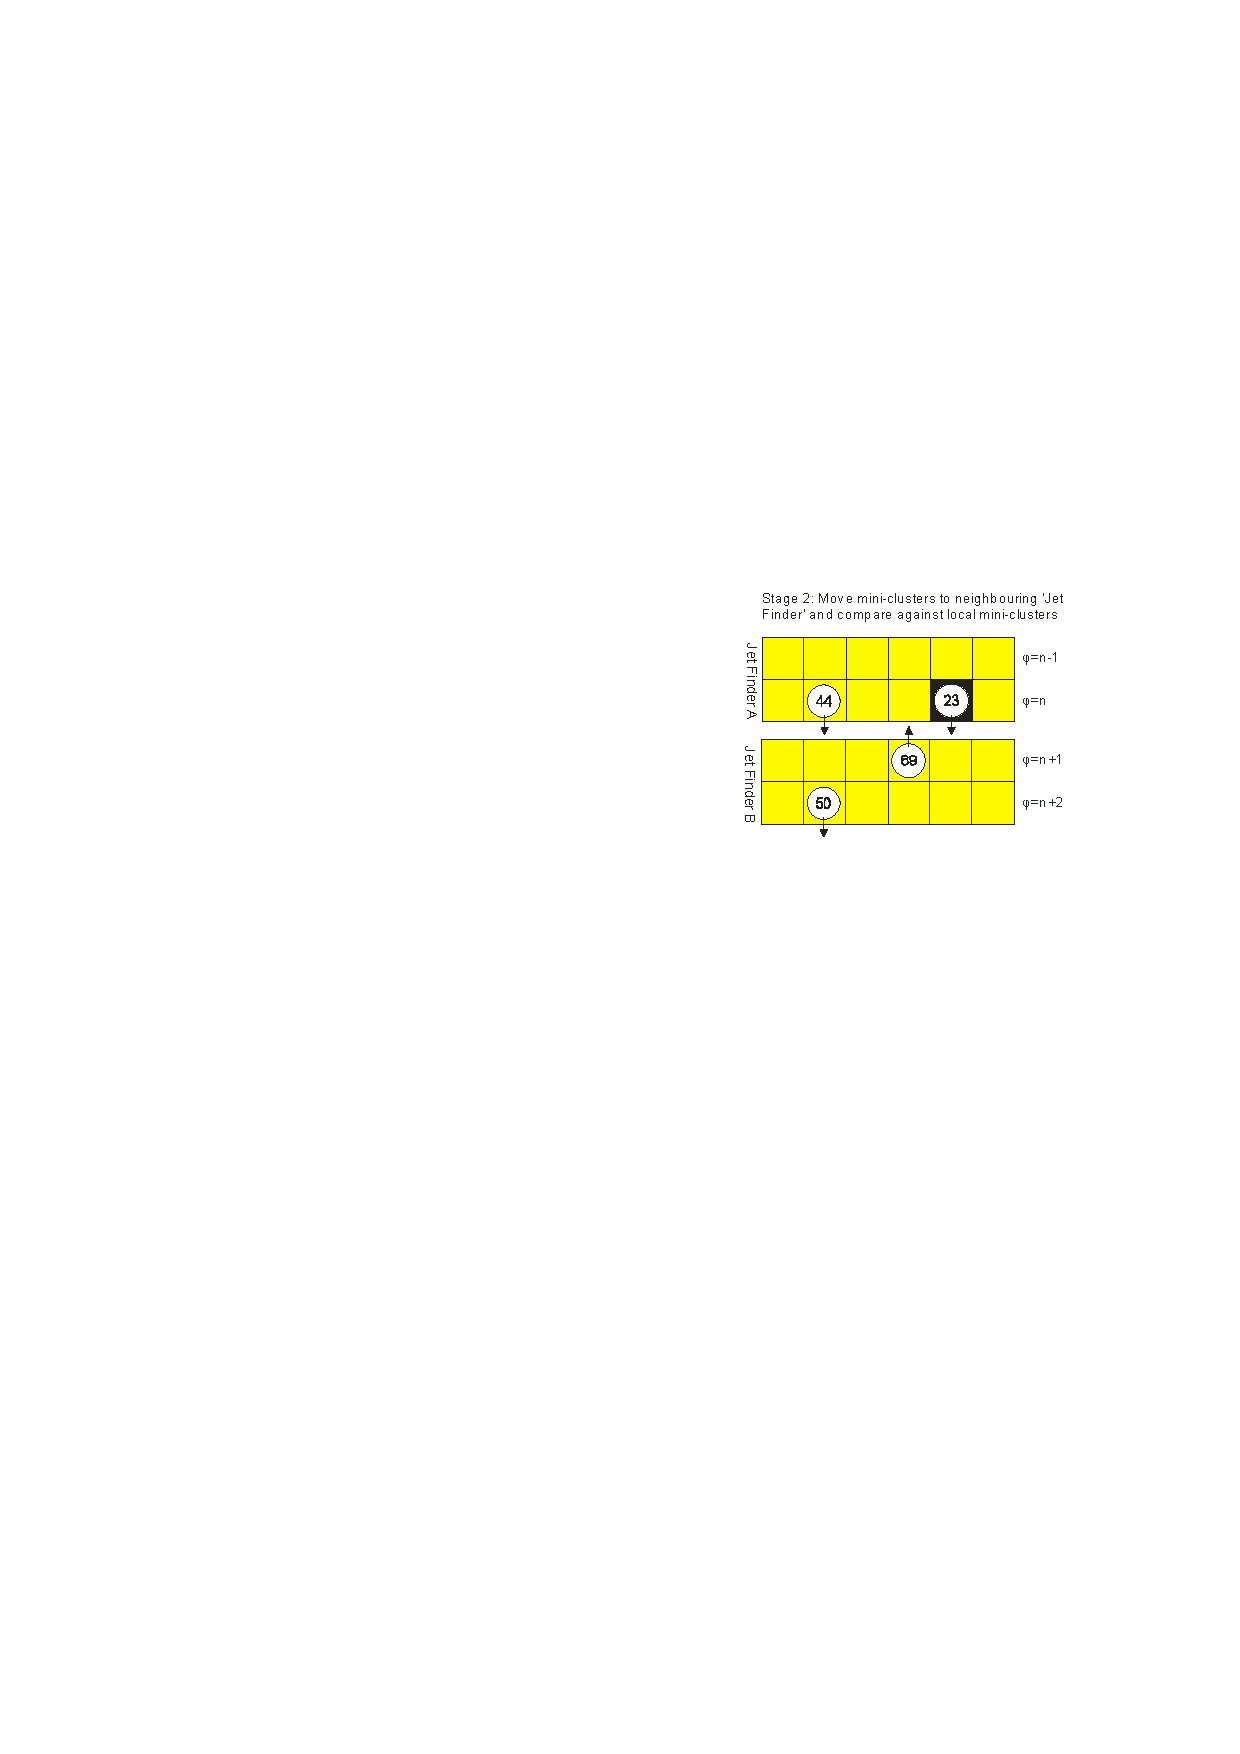
\includegraphics[width = 1.0\linewidth]{plots/l1_stage2.pdf}
\end{minipage}
\quad\quad
\begin{minipage}[b]{0.46 \linewidth}
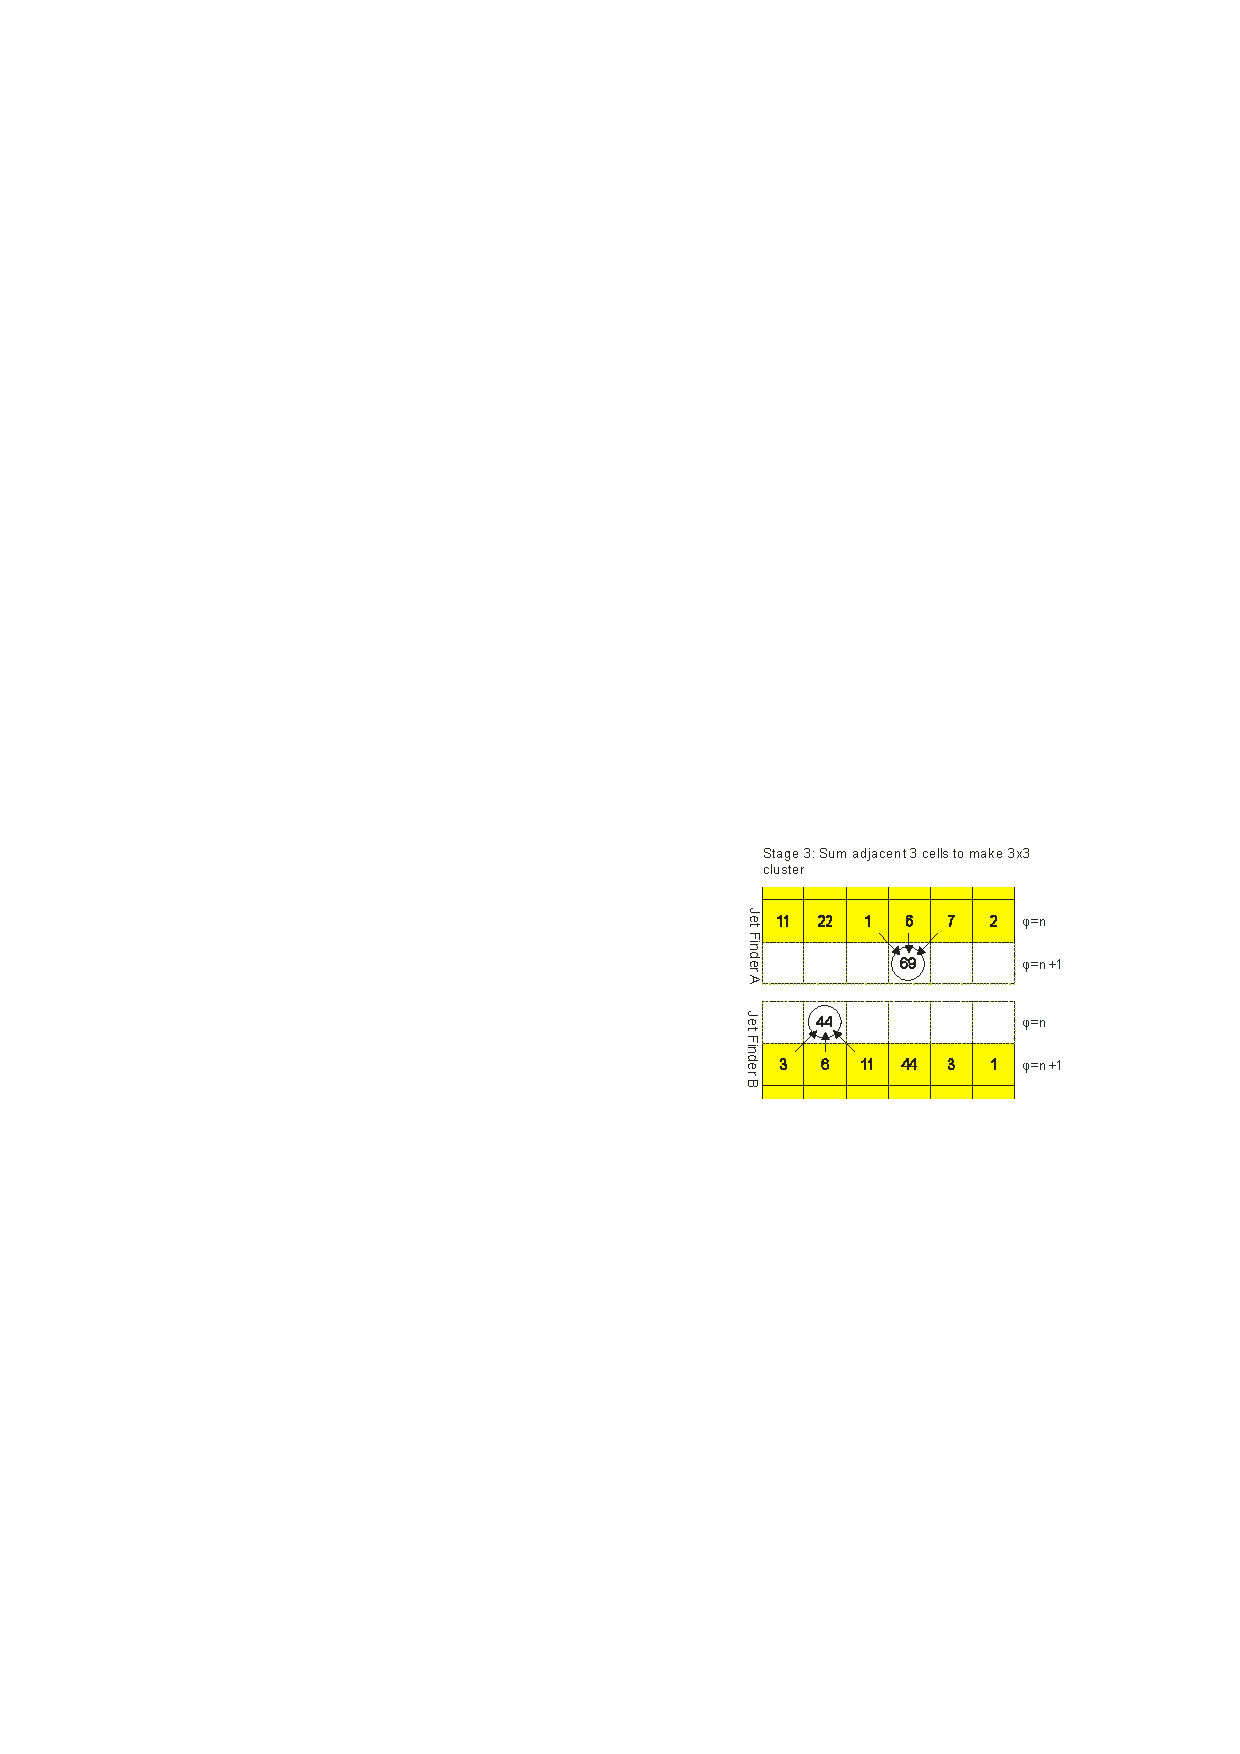
\includegraphics[width = 1.0\linewidth]{plots/l1_stage3.pdf}
\end{minipage}
\quad
\begin{minipage}[b]{0.46 \linewidth}
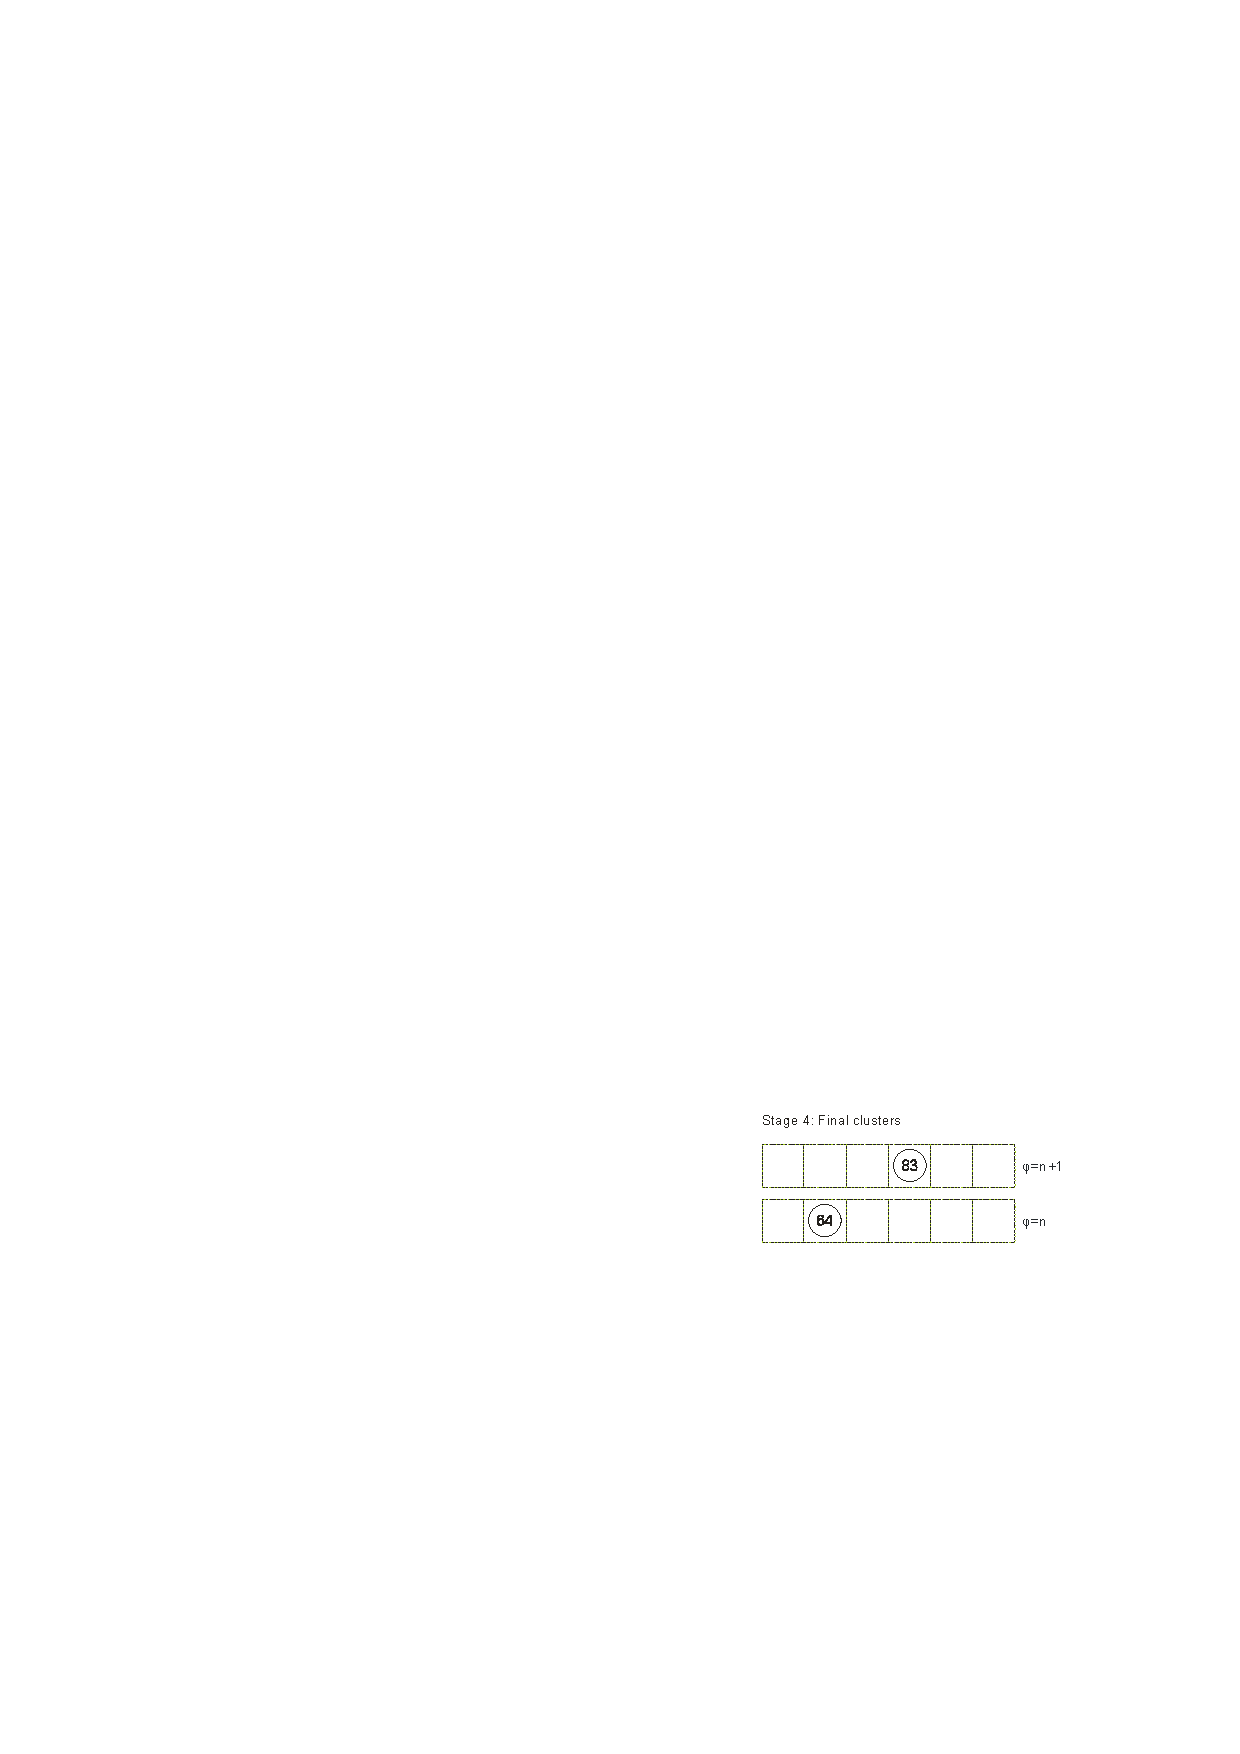
\includegraphics[width = 1.0\linewidth]{plots/l1_stage4.pdf}
\end{minipage}
\quad
\caption[The four stages of the jet clustering method.]{The four stages of the jet clustering method. Each numerical value represents an energy sum deposited within the trigger tower. Only 6 cells in $\eta$ are shown, but there exist 11 cells per half detector. 18 $\phi$ strips operate in parallel across the detector to perform jet clustering \cite{Iles:1028171}.}
\label{fig:l1_stage} 
\end{figure}


Within the $|\eta| <$ 3 region, the \ac{GCT} also determines whether a jet is to be classified as a $\tau$ or central jet. The hadronic decay modes of the $\tau$ typically contain one or three isolated pions, thus leading to more collimated energy deposits with fewer constituents than non-\tau jets. Therefore, for a jet candidate to be classed as a $\tau$ jet, up to a maximum of one of the eight calorimeter regions neighbouring the central jet seed is permitted to have a transverse energy, $\et$, above some programmable isolation threshold. Due to the granularity of the \ac{CMS} detector at high $\eta$, this check can only occur in the barrel and therefore $\tau$ jets can only be identified within the central region.

Jets found between $3.0<|\eta|<5.0$ are classified as forward jets, whereas those with $|\eta|<3.0$ are classified as either a central or $\tau$-jet. The four clustered jets with the highest transverse energy in each category (central, forward and $\tau$-jet) are further passed through \acf{LUT}s, which apply a programmable $\eta-$dependent jet energy scale correction. Finally these jet objects are passed to the \ac{GT} to make \L1 trigger decisions.

The performance of \L1 jets within the following sections are evaluated with respect to offline jets, which are taken from the standard \Calo jet and the \PF jet reconstruction algorithms of \ac{CMS}. These reconstructed offline jets are corrected for pile-up and detector effects as described in Section (\ref{subsec:cmsobjects-jets}). A moderate level of noise rejection is applied to the offline jets by selecting jets passing the ``loose'' identification criteria for both \Calo and \PF. These jet criteria are listed in  Table \ref{tab:calojetid} and Table \ref{apptab:pfjetid} respectively. 


\subsection{Measurement of \L1 Single-Jet Trigger Efficiencies}
\label{subsec:l1jettrigeff}

The efficiency of a \L1 single-jet trigger at an offline reconstructed jet \et is determined from events in a sample containing at least a single reconstructed offline jet. It is defined as, the fraction of events where the leading offline jet is matched to a L1 central or $\tau$ jet that also has a measured \L1 energy above the trigger threshold being benchmarked.

A match is determined by comparing the \L1 and reconstructed offline jets spatially in $\eta - \phi$ space.  The $\Delta R$ separation between the highest offline reconstructed jet  ($\et > 10$ \GeV and $\lvert\eta\rvert<3$) and each \L1 jet in the event is calculated. A match is made to the \L1 jet with the minimum $\Delta R$ to the reconstructed jet and if it also lie within a cone of $\Delta R < 0.5$ of the offline jet. 

The matching efficiency for this procedure is found to be above 99$\%$ for an offline jet threshold above 30(45) GeV for the run 2012B(C) data taking period (see Appendix \ref{app:jetmatching}).

Each efficiency curve is fitted with a function which is the cumulative distribution function of an \acf{EMG} distribution:
\begin{eqnarray}
f(x; \mu, \sigma, \lambda) = \frac{\lambda}{2} \cdot e^{\frac{\lambda}{2}(2 \mu + \lambda \sigma^2 - 2 x)} \cdot \textrm{erfc}\left( \frac{\mu + \lambda \sigma^2 - x}{\sqrt{2} \sigma}\right)
\label{eq:emg}
\end{eqnarray}
where \textrm{erfc} is the complementary error function defined as:
$$ \textrm{erfc}(x) = 1 - \textrm{erf}(x) = \frac{2}{\sqrt{\pi}} \int_{x}^{\infty} e^{-t^2} dt.$$

In this functional form, the parameter $\mu$ determines the point of 50\% of the plateau efficiency, and $\sigma$ gives the resolution. This parametrisation is used to benchmark the efficiency at the plateau, the turn-on points and resolution for each L1 Jet trigger. The choice of function is purely empirical. Previous studies used the error function alone, which described the data well at high threshold values but could not describe the efficiencies well at lower thresholds \cite{L1JEC}.

The efficiency turn-on curves for various \L1 jet thresholds are evaluated as a function of the offline reconstructed jet E$_{T}$ for central jets with $| \eta | < 3$. These are measured using single isolated $\mu$ triggers which are unbiased to the hadronic triggers under study as they are triggered on muon objects. Events are selected to make sure the muon does not overlap with a jet $\Delta R (\mu,jet) > 0.5$, causing a discrepancy in the measurement of the calorimetric energy.

The efficiency is calculated with respect to offline \Calo and \PF Jets in Figure  \ref{fig:l1jet-calopf-mu}. Table \ref{tab:l1jettable} shows the values of these parameters, calculated for three \L1 single jet triggers measured from 2012 8 \TeV data. Benchmarked are the \et 16, \et 36 and \et 92 single jet triggers which are given in the table with their trigger path names \texttt{L1\_SingleJet16}, \texttt{L1\_SingleJet32} and \texttt{L1\_SingleJet92} respectively.

\FloatBarrier
\begin{figure}[ht]
\centering
\begin{minipage}[b]{0.46 \linewidth}
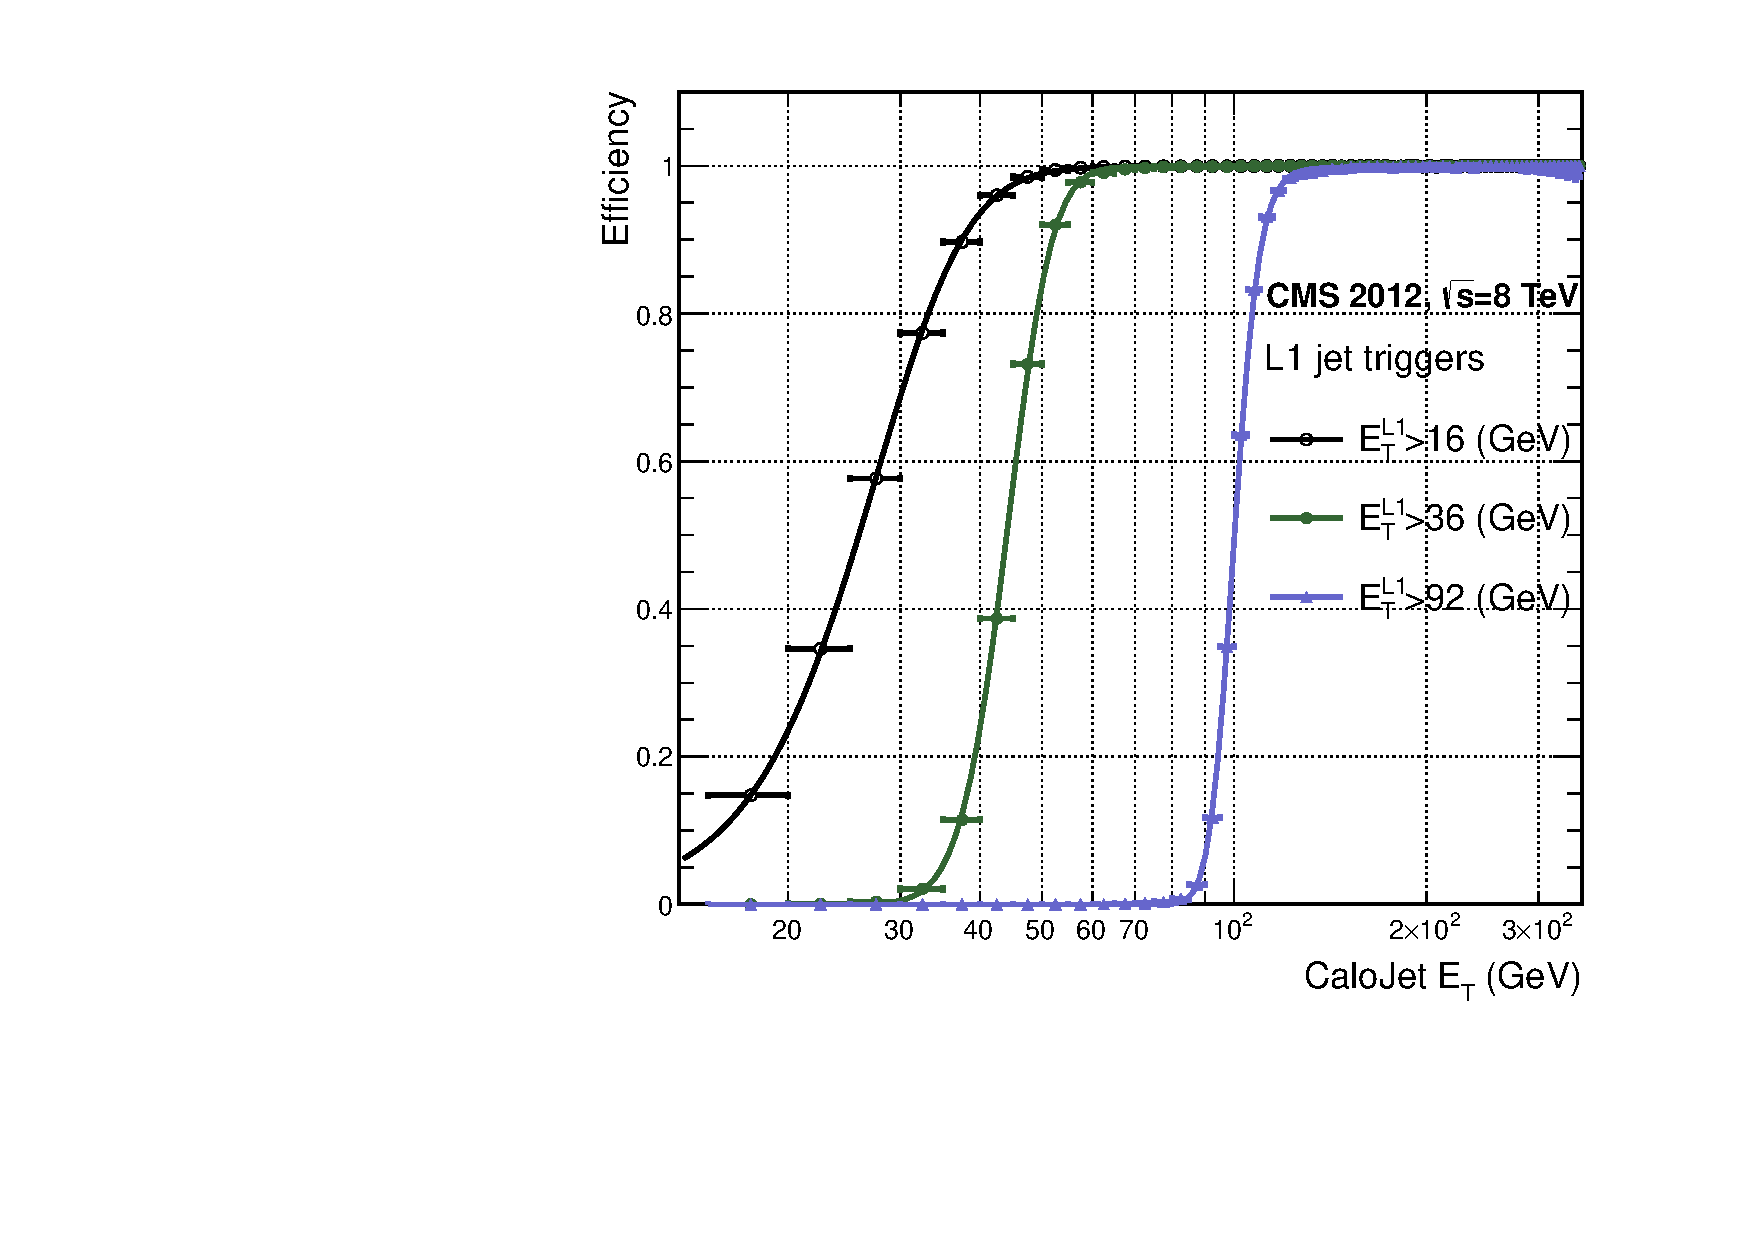
\includegraphics[width = 1.0\linewidth]{plots/jetpt_RunC.pdf}
\end{minipage}
\quad
\begin{minipage}[b]{0.46 \linewidth}
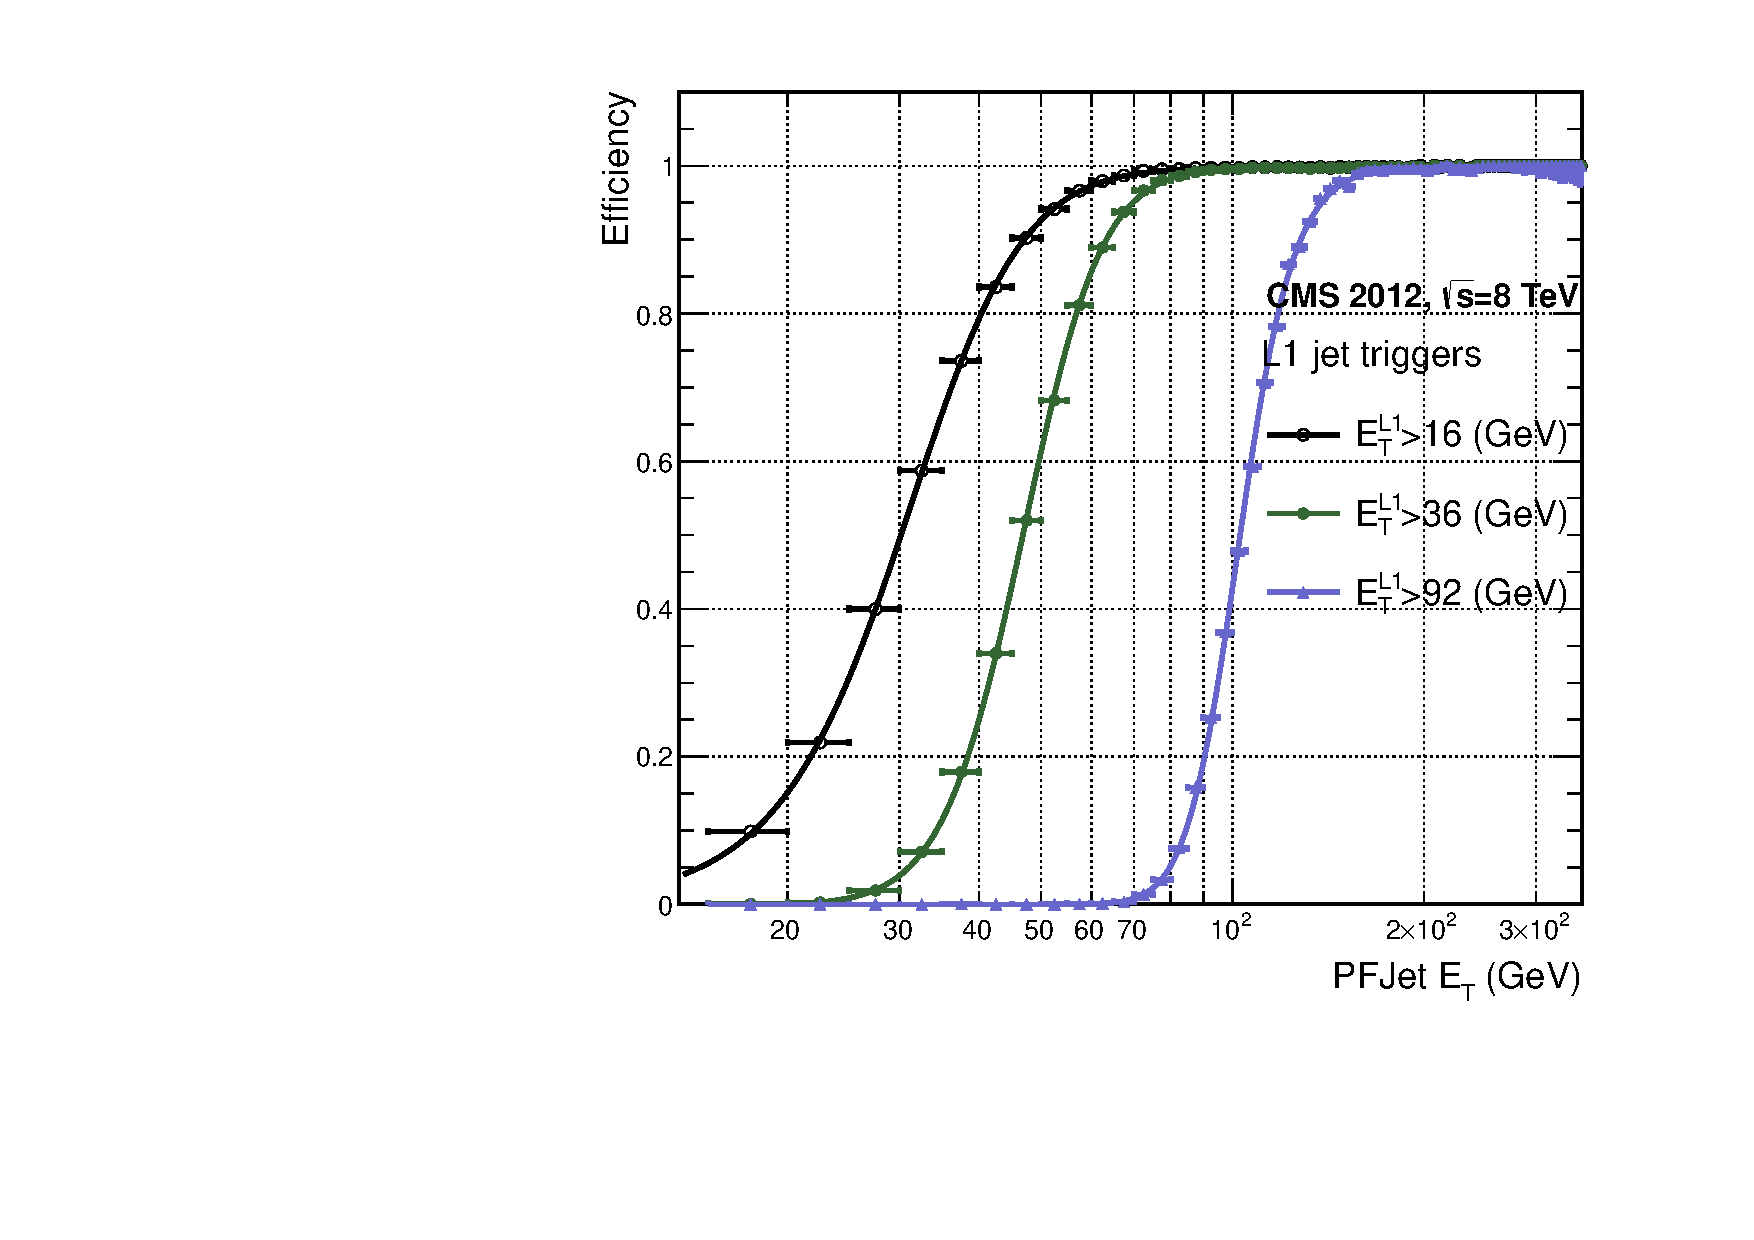
\includegraphics[width = 1.0\linewidth]{plots/jetpt_RunC_PF.pdf}
\end{minipage}
\quad
\caption[L1 jet efficiency turn-on curves as a function of the offline CaloJet and PFJet $\et$. ]{L1 jet efficiency turn-on curves as a function of the offline CaloJet $\et$ (left) and PFJet $\et$ (right), measured in 2012 Run Period C data and collected with an isolated single $\mu$ data sample.}
\label{fig:l1jet-calopf-mu} 

\end{figure}

\begin{table}
\begin{center}
\footnotesize
\begin{tabular*}{0.75\textwidth}{@{\extracolsep{\fill}}c|cc|cc}
\hline
\multicolumn{1}{c}{}& \multicolumn{2}{c}{Calo} & \multicolumn{2}{c}{PF} \\ 
\multicolumn{1}{c}{Trigger} & $\mu$ & \multicolumn{1}{c}{$\sigma$} & $\mu$ & $\sigma$ \\ \hline\hline
\texttt{L1\_SingleJet16} & 21.09 $\pm$ 0.03 & 7.01 $\pm$ 0.02 & 22.17 $\pm$ 0.04 & 7.83 $\pm$ 0.03 \\ 
\texttt{L1\_SingleJet36} & 41.15 $\pm$ 0.05 & 5.11 $\pm$ 0.02 & 39.16 $\pm$ 0.06 & 8.04 $\pm$ 0.03 \\ 
\texttt{L1\_SingleJet92} & 95.36 $\pm$ 0.13 & 5.62 $\pm$ 0.03 & 90.85 $\pm$ 0.19 & 11.30 $\pm$ 0.10  \\ 
\end{tabular*}
\end{center}

\caption[Results of a cumulative \ac{EMG} function fit to the turn-on curves for \L1 single jet triggers in 2012 Run Period C.]{Results of a cumulative \ac{EMG} function fit to the turn-on curves for \L1 single jet triggers in run 2012 Run Period C, measured in an isolated $\mu$ data sample. The turn-on point, $\mu$, and resolution, $\sigma$, of the L1 jet triggers are measured with respect to offline Calo Jets (left) and PF Jets (right). Errors quoted are statistical only.}
\label{tab:l1jettable}
\end{table}

The results from the \L1 single jet triggers shows good performance for both \Calo and \PF jets. A better resolution is observed for \Calo jets with respect to \L1 single-jet quantities. This effect is due to \Calo jet reconstruction using the same detector subsystems (\ECAL and \HCAL only) as the \L1 jets. 

In contrast the \PF jet reconstruction algorithm additionally utilises tracker and muon information, resulting in a poorer compatability between the jet energy sums when directly compared to \L1 jet objects. 

\section{\L1 Trigger Performance After the Introduction of a \L1 Jet Seed}
\label{subsec:l1jetseedpu}

Between run period B and C of the 2012 data taking period, a jet seed threshold was introduced into the \L1 jet clustering algorithm. There was previously no direct requirement made on this energy deposited in this central seed region. 

The introduction of a jet seed threshold required that the central region have an uncorrected energy deposit of $\et \geq 5$ \GeV. This value was motivated by studies of the effect that different jet seed thresholds had upon the trigger cross-sections and efficiencies of various \theht, single jet and multi-jet triggers. It was found that the 5 \GeV threshold gave large reductions in trigger cross-sections (the rate at which a trigger fires) particularly in the case of multi-jet and \theht triggers, whilst having a small impact on the measured efficiencies of these triggers \cite{Shorney-Mathias:1641954}.

Its main purpose was to counteract the effects of high pile up running conditions which create a large number of soft non-collimated jets, that are then added to the jets from the primary interaction or other soft jets from other secondary interactions \cite{L1bryn}. This in turn causes a large increase in the number of \L1 jets created from each collision, leading to an increase in the likelihood that the event causes the \L1 trigger to fire. 

The effect of the introduction of this jet seed threshold between these two run periods is benchmarked through a comparison of the efficiency vs \et of the \L1 jet triggers with respect to offline Calo jets and is shown in Figure \ref{fig:l1jetseeds}. The single jet triggers \et 36 and \et 92 are used for the purpose of this comparison.

The \L1 $H_{T}$ trigger efficiency is also measured at two thresholds of 100 \GeV and 150 \GeV, which is shown in Figure \ref{fig:l1jetseedht}. This is also represented in the respective  trigger path names \texttt{L1HTT100} and \texttt{L1HTT150}. The \L1 \theht sum is compared against the offline $\theht$ constructed from Calo jets with $\et \geq$ 40 \GeV. This requirement is imposed to account for the relative difference between uncorrected jet energy deposits within the \ac{GCT} used to calculate the \L1 \theht sum, and those same deposits after full object reconstruction has occurred.

To negate any effects from different pile-up conditions in the run periods, the efficiencies are measured in events which contain between 15 and 20 primary vertices, as defined by Table (\ref{tab:primaryvertices}). This range represents the mean number of primary vertices observed during the entire \com = 8 \TeV run period.

\begin{table}[H]
\footnotesize
\begin{center}
\begin{tabulary}{0.80\textwidth}{p{3cm}L}
\cline{1-2}
\multicolumn{2}{l}{Good primary vertex requirement} \\
Variable & Definition \\ 
\hline\hline
$N_{dof} > 4$ \qquad\qquad\qquad & The number of degree of freedom, from the vertex fit to compute the best estimate of the vertex parameters. \\
$\vert \Delta z_{vtx} \vert < 24$cm &  The distance, $\vert\Delta z_{vex}\vert$, to the position of the closest \ac{HLT} primary vertex. \\ 
 $\rho < 2$cm & The perpendicular distance of track position to the beam spot. \\
\cline{1-2}
\end{tabulary}
\end{center}
\caption[Criteria for a vertex in an event to be classified as a 'good' reconstructed primary vertex.]{Criteria for a vertex in an event to be classified as a 'good' reconstructed primary vertex.}
\label{tab:primaryvertices}
\end{table}


\begin{figure}[ht]
\centering
\begin{minipage}[b]{0.46 \linewidth}
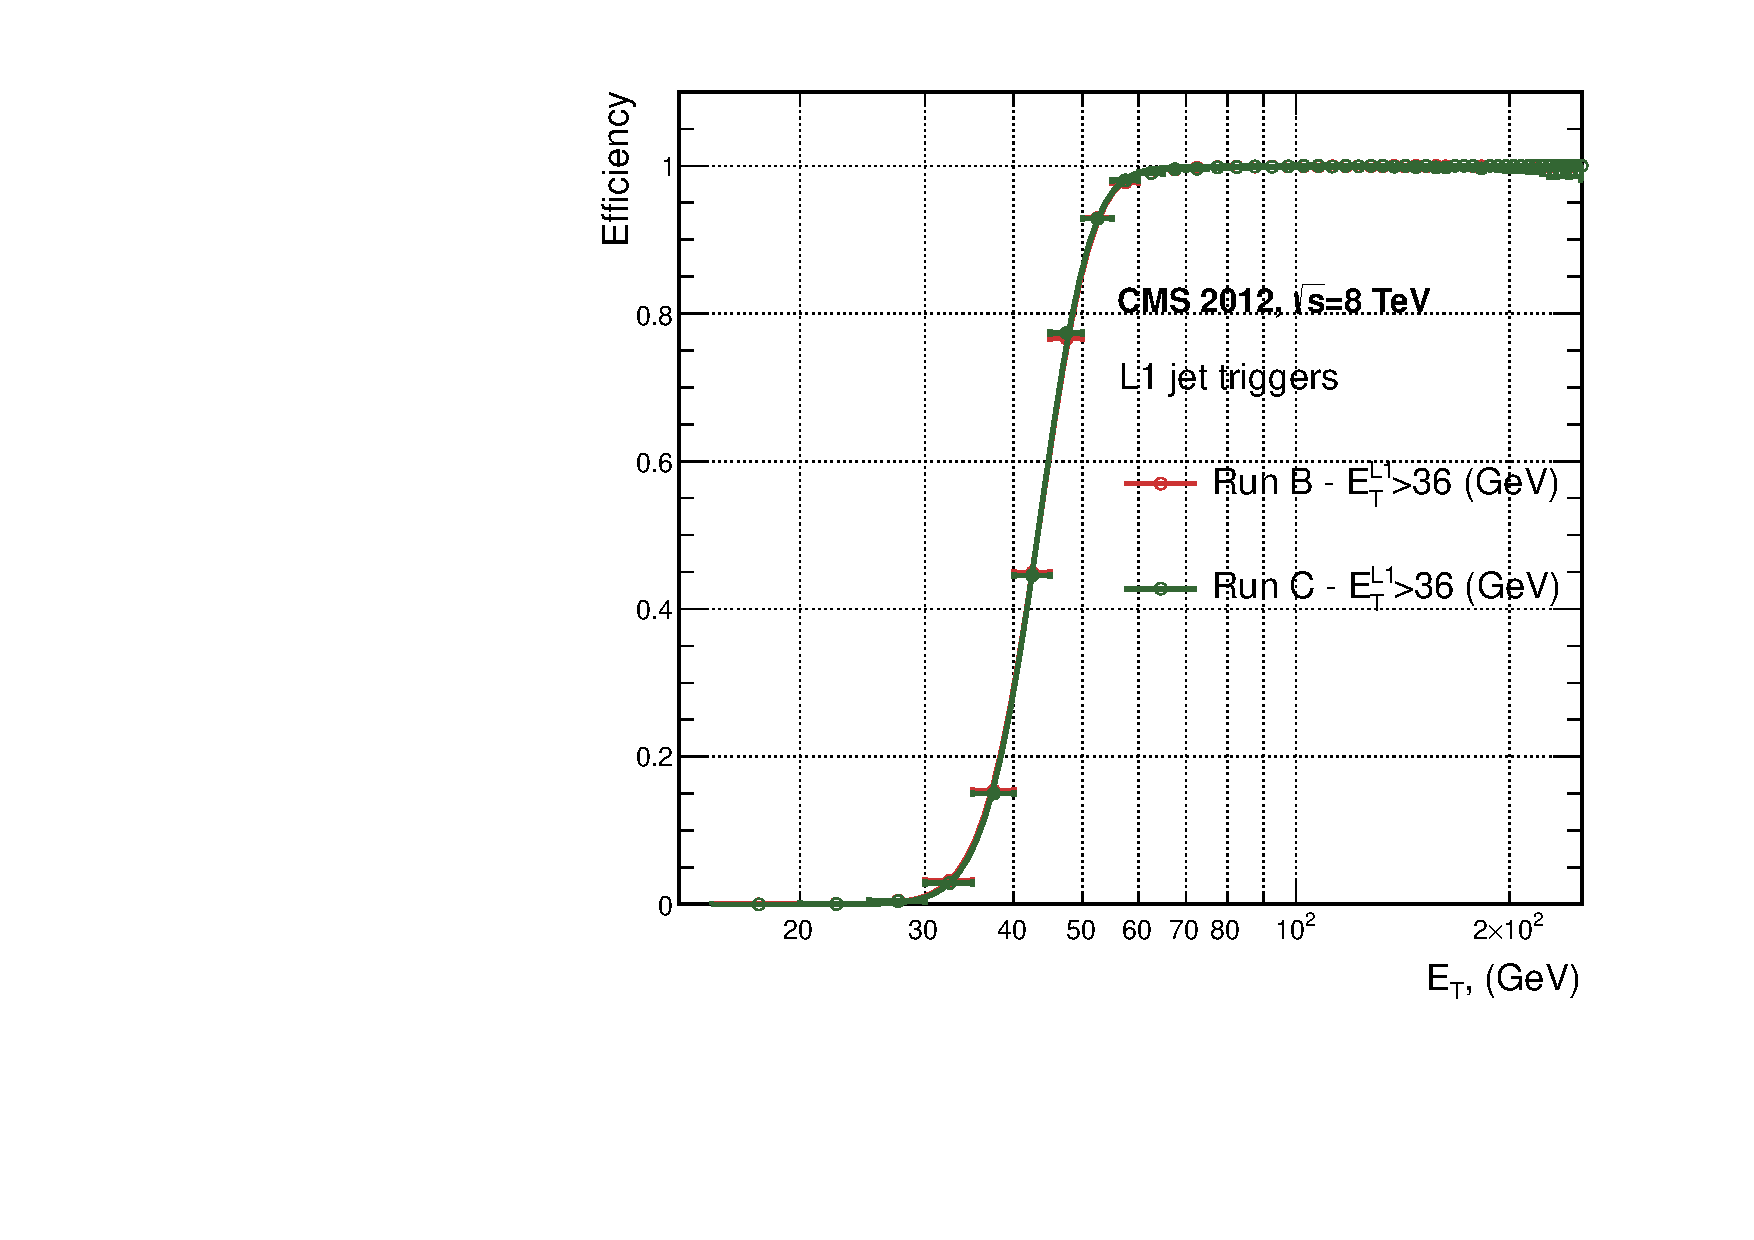
\includegraphics[width = 1.0\linewidth]{plots/jetseed_36.pdf}
\end{minipage}
\quad
\begin{minipage}[b]{0.46 \linewidth}
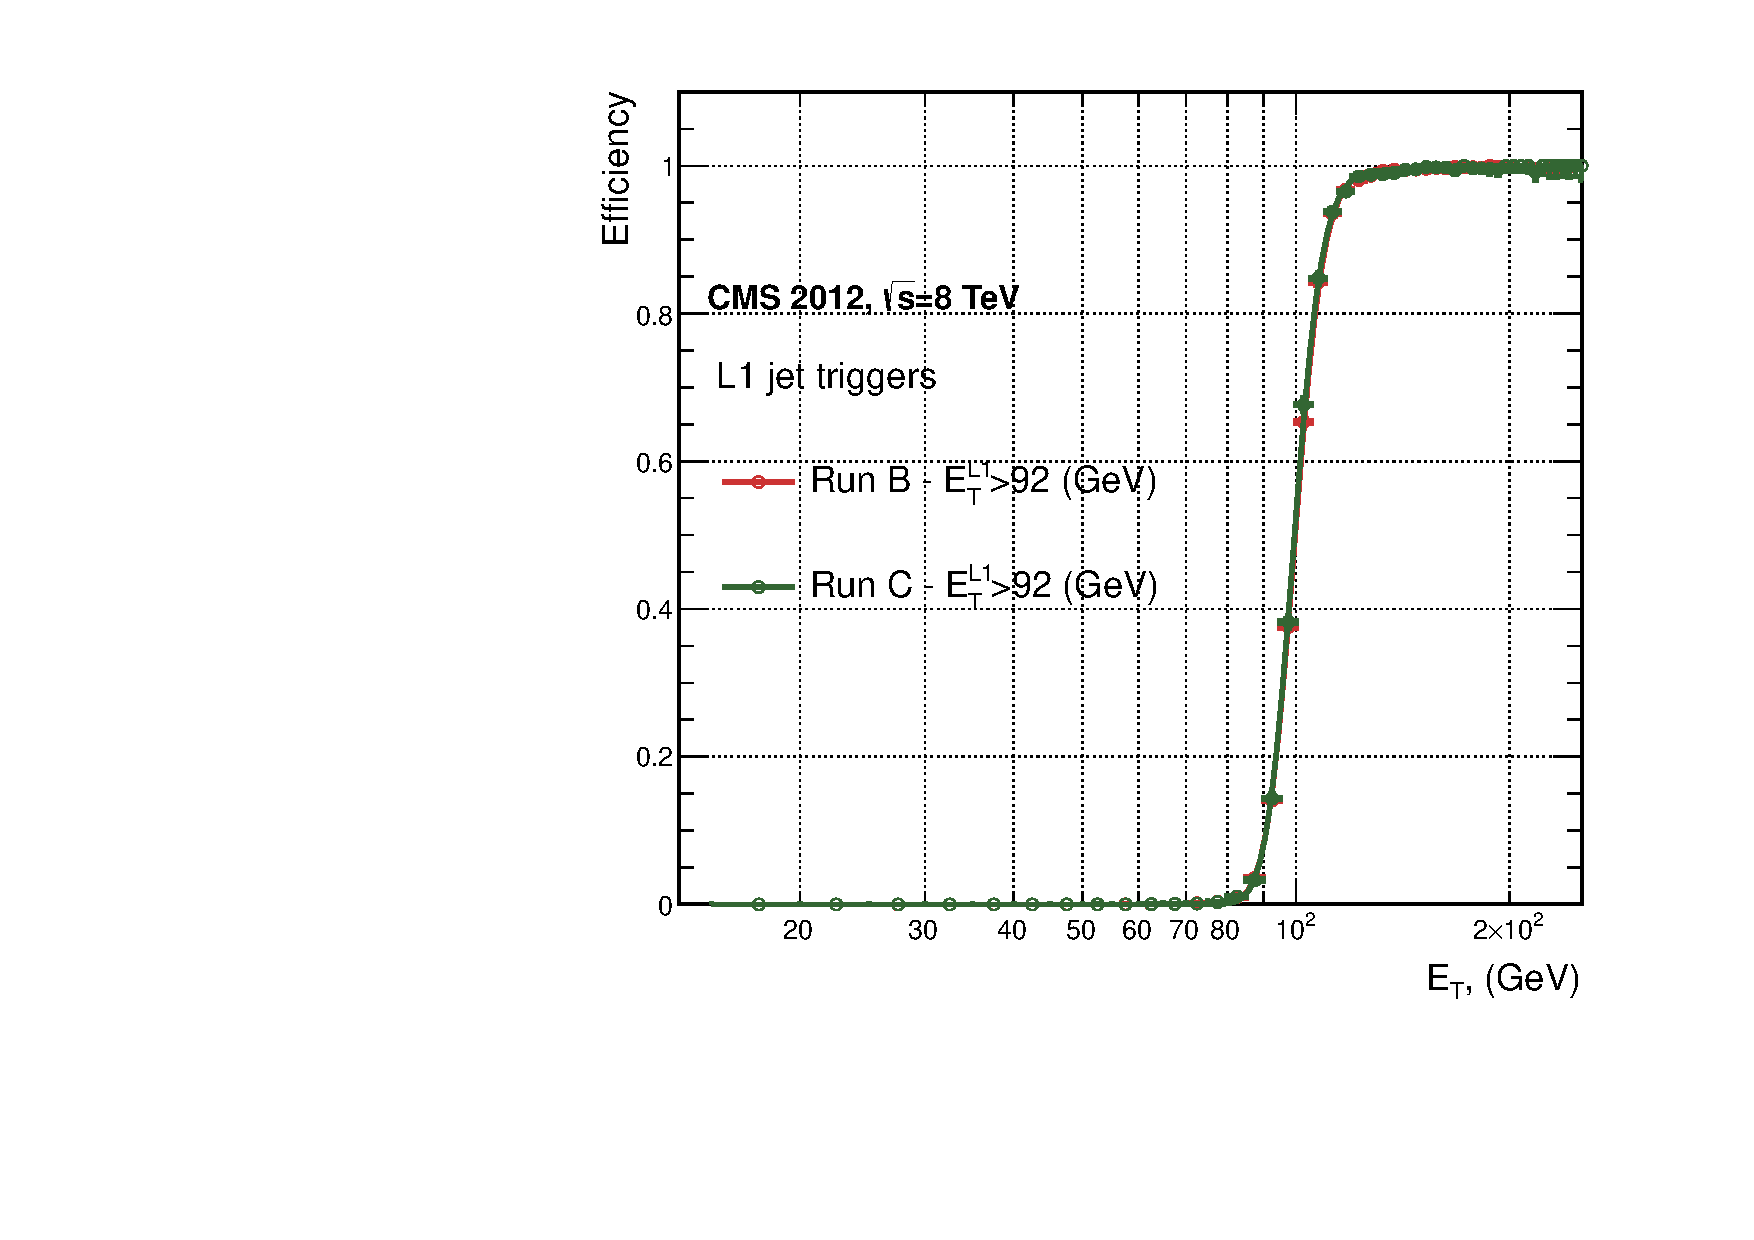
\includegraphics[width = 1.0\linewidth]{plots/jetseed_92.pdf}
\end{minipage}
\quad
\caption[L1 jet efficiency turn-on curves as a function of the offline CaloJet E$_{T}$ for the 2012 run period B and C.]{L1 jet efficiency turn-on curves as a function of the offline CaloJet E$_{T}$, measured for the \texttt{L1\_SingleJet36} and \texttt{L1\_SingleJet92} trigger paths in 2012 run period B and C collected with an isolated single $\mu$ sample.}
\label{fig:l1jetseeds} 
\end{figure}

\begin{figure}[ht]
\centering
\begin{minipage}[b]{0.46 \linewidth}
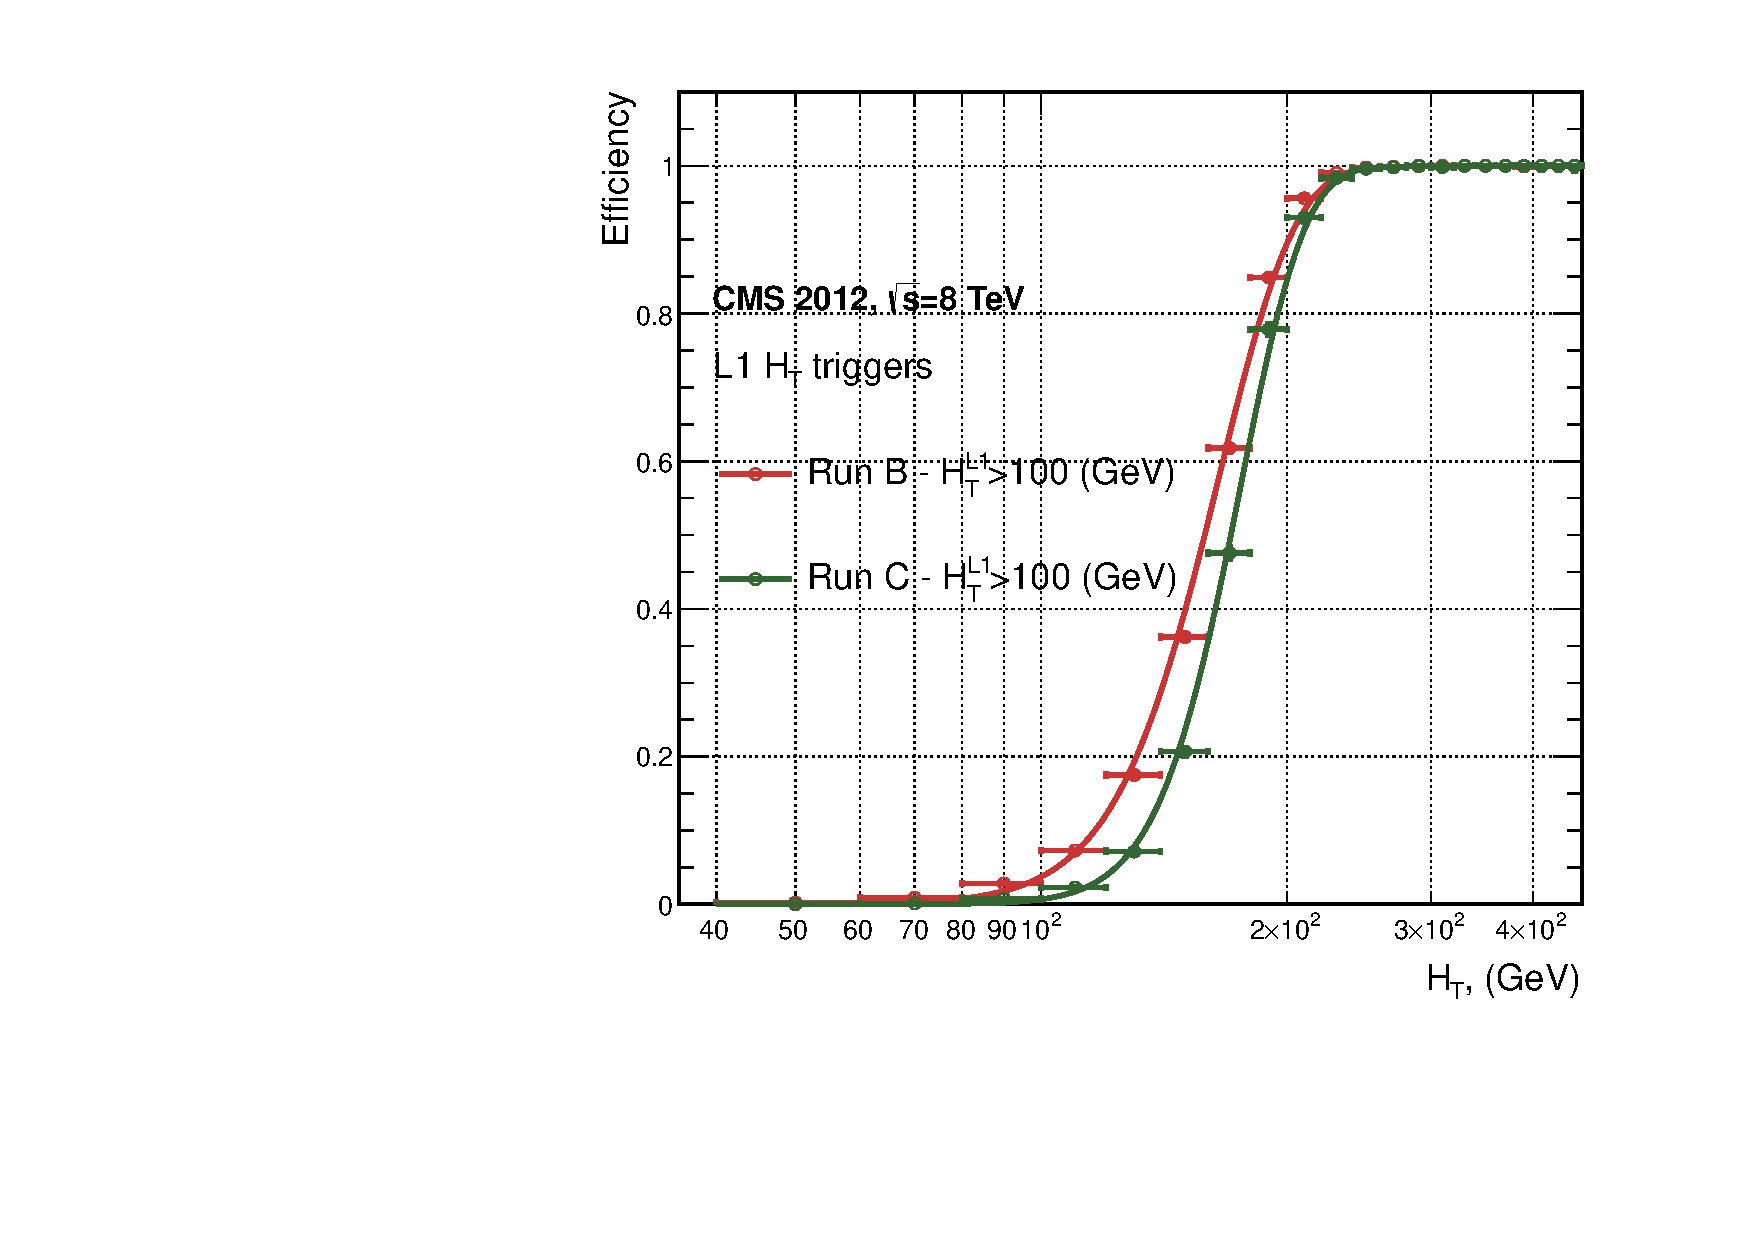
\includegraphics[width = 1.0\linewidth]{plots/jetseed_ht100.pdf}
\end{minipage}
\quad
\begin{minipage}[b]{0.46 \linewidth}
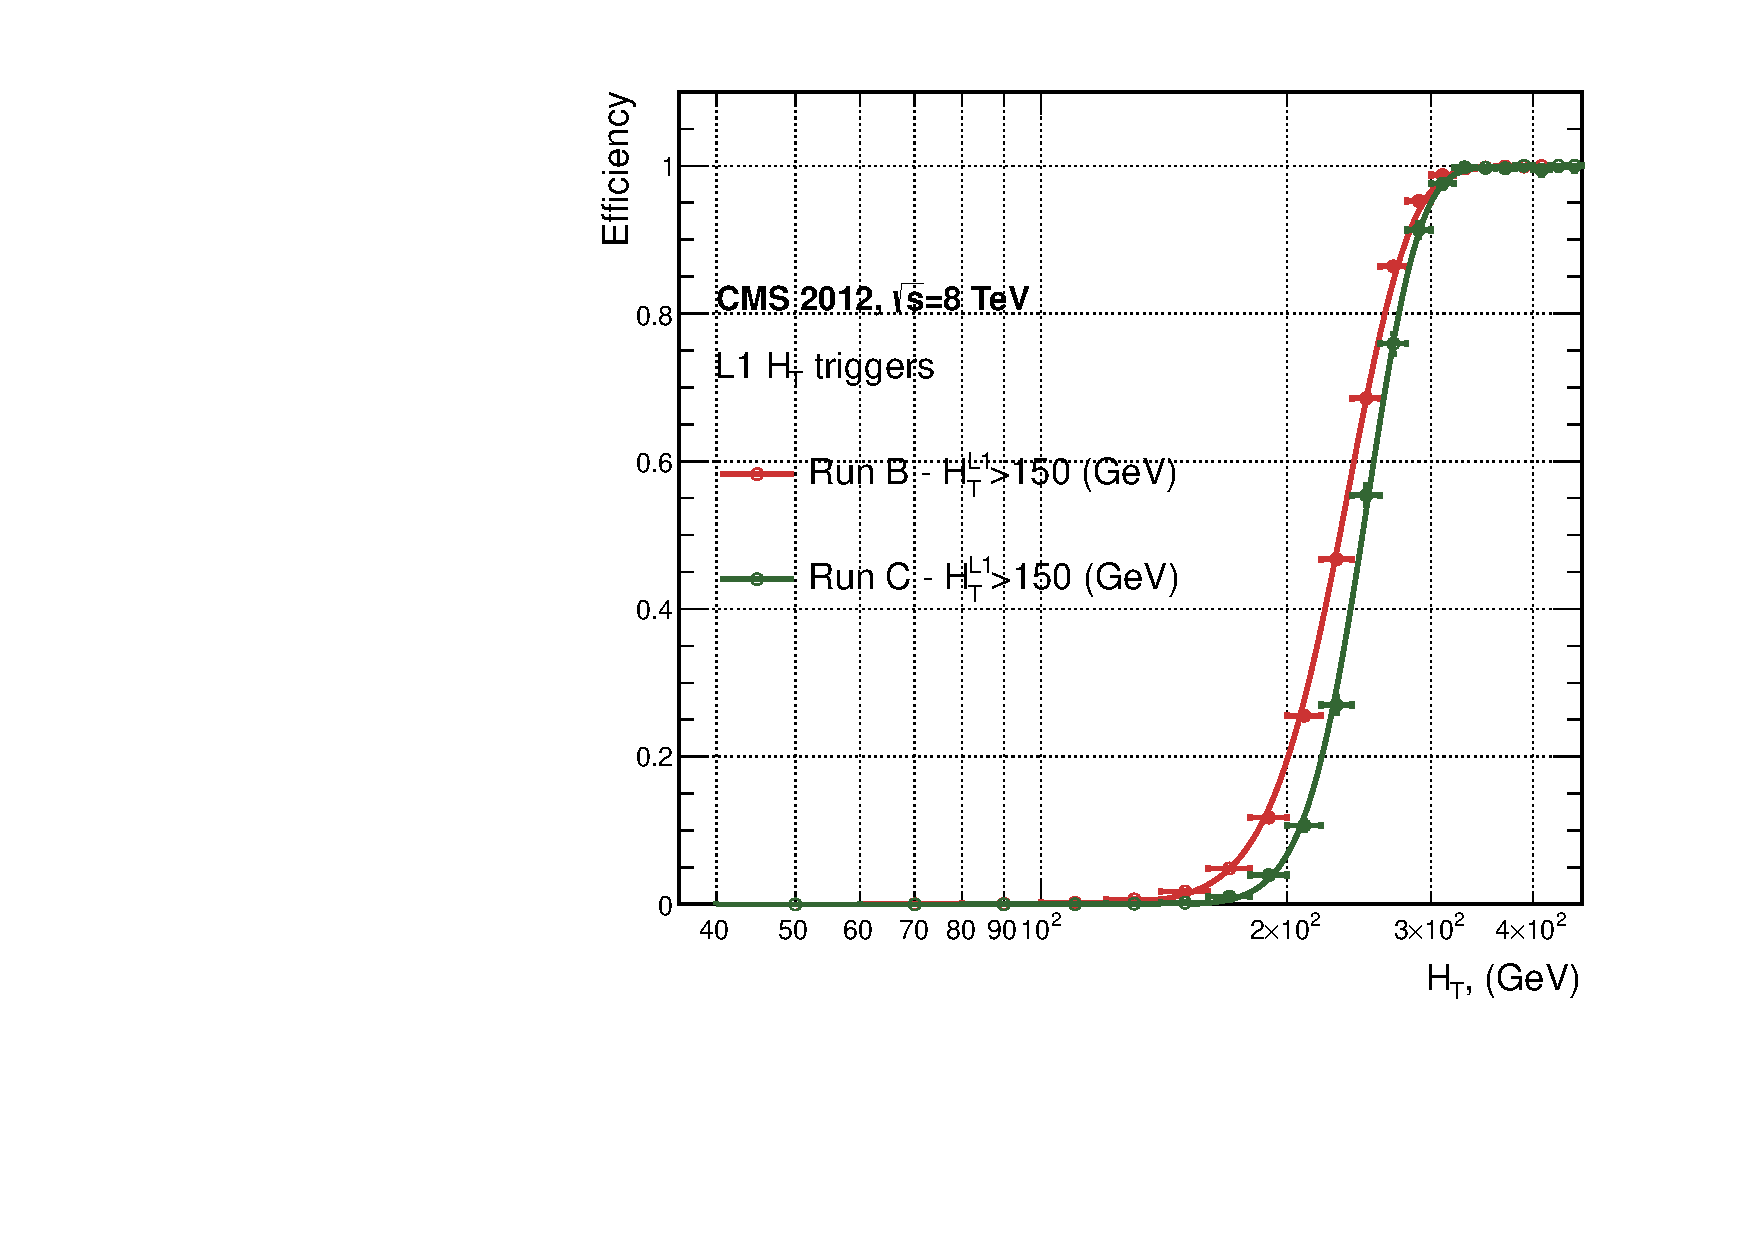
\includegraphics[width = 1.0\linewidth]{plots/jetseed_ht150.pdf}
\end{minipage}
\quad
\caption[\L1 $\theht$ efficiency turn-on curves as a function of the offline CaloJet $\theht$.]{\L1 $\theht$ efficiency turn-on curves as a function of the offline CaloJet $\theht$, measured for the \texttt{\L1$\theht$T100} and \texttt{L1HTTT150} trigger paths during the run 2012 B and C, collected using an isolated single $\mu$ triggered sample.}
\label{fig:l1jetseedht} 
\end{figure}

It can be seen that the performance of the $E_{T} > 36,92 \GeV$ single jet triggers are almost identical, with the jet seed having no measurable effect on these triggers as shown in Table \ref{tab:l1jetseedtable}. 

\begin{table}[h!]
\begin{center}
\footnotesize
\begin{tabular*}{0.75\textwidth}{@{\extracolsep{\fill}}c|cc|cc}
\hline
\multicolumn{1}{c}{}& \multicolumn{2}{c}{2012B} & \multicolumn{2}{c}{2012C} \\ 
\multicolumn{1}{c}{Trigger} & $\mu$ & \multicolumn{1}{c}{$\sigma$} & $\mu$ & $\sigma$ \\ \hline\hline
\texttt{L1\_SingleJet36} & 40.29 $\pm$ 0.04& 5.34 $\pm$ 0.02 & 40.29 $\pm$ 0.11 & 5.21 $\pm$ 0.05 \\ 
\texttt{L1\_SingleJet92} & 94.99 $\pm$ 0.09 & 5.93 $\pm$ 0.06 & 94.82 $\pm$ 0.29 & 5.74 $\pm$ 0.18 \\ 
\end{tabular*}
\end{center}
\caption[Results of a cumulative \ac{EMG} function fit to the turn-on curves for \L1 single jet triggers in the 2012 run period B and C.]{Results of a cumulative \ac{EMG} function fit to the turn-on curves for \L1 single jet triggers in the 2012 run period B and C, preselected on an isolated muon trigger. The turn-on point $\mu$ and resolution $\sigma$ of the L1 jet triggers are measured with respect to offline Calo Jets in run B (left) and run C (right). }
\label{tab:l1jetseedtable}

\end{table}

In the case of the $\theht$ triggers, without the jet seed threshold a large increase in the trigger cross-section during high luminosity collisions will occur. The low energy threshold requirement for a jet to be clustered and added to the \L1 $\theht$ sum, will allow many soft jets from other secondary interactions to enter the calculation. The introduction of the jet seed threshold prevents the clustering of many of these diffuse low $\et$ pile-up jets, thus lowering the \L1 \ac{GCT} $\theht$ calculation. Resultantly, different behaviours for the trigger turn-ons after the introduction of the jet seed threshold are expected for these triggers. 

The $\mu$ values are observed to reside at higher \theht for both \theht trigger thresholds indicating a slower turn-on, whilst a better resolution is observed after the introduction of the jet seed threshold. These values can be found within Table \ref{tab:l1jetseedtableHT}.

\begin{table}[h!]
\begin{center}
\footnotesize
\begin{tabular*}{0.75\textwidth}{@{\extracolsep{\fill}}c|cc|cc}
\hline
\multicolumn{1}{c}{}& \multicolumn{2}{c}{2012B} & \multicolumn{2}{c}{2012C} \\ 
\multicolumn{1}{c}{Trigger} & $\mu$ & \multicolumn{1}{c}{$\sigma$} & $\mu$ & $\sigma$ \\ \hline\hline
\texttt{L1HTT100} & 157.5 $\pm$ 0.08 & 32.9 $\pm$ 0.08 & 169.8 $\pm$ 0.08 & 28.7 $\pm$ 0.03 \\ 
\texttt{L1H1T150} & 230.9 $\pm$ 0.02 & 37.3 $\pm$ 0.01 & 246.4 $\pm$ 0.16 & 31.8 $\pm$ 0.05 \\ 
\end{tabular*}
\end{center}
\caption[Results of a cumulative \ac{EMG} function fit to the turn-on curves for $\theht$ in 2012 run period B and C.]{Results of a cumulative \ac{EMG} function fit to the turn-on curves for $\theht$ in run 2012 B and C, preselected on an isolated single $\mu$ trigger. The turn-on point $\mu$ and resolution $\sigma$ of the \L1 $\theht$ triggers are measured with respect to offline $\theht$, formed from CaloJets with a $\et \geq 40$  in run period B (left) and C (right). }
\label{tab:l1jetseedtableHT}
\end{table}

Despite this slight increase in the turn-on point of the \theht triggers, a large reduction in the trigger cross-section is achieved for all \theht triggers. As an example, the expected trigger cross-section for the \texttt{L1HTT150} trigger as a function of instantaneous luminosity is shown in Figure \ref{fig:l1rateplot}. 

\begin{figure}[ht!]
\centering
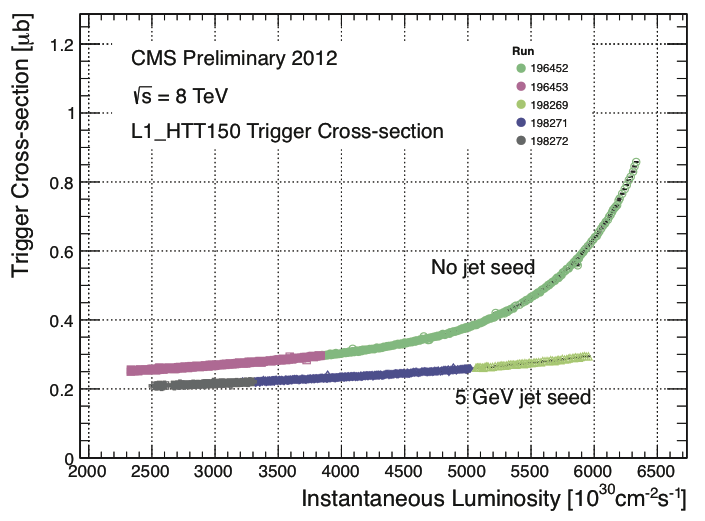
\includegraphics[scale=0.71]{plots/l1rateplot.pdf}
\caption[Trigger cross section for the \texttt{L1HTT150} trigger path. ]{Trigger cross section for the \texttt{L1HTT150} trigger path. Showing that a 5 \GeV jet seed threshold dramatically reduces the dependance of cross section on the instantaneous luminosity for \L1 $\theht$ triggers \cite{l1ratebrooke}.}  
\label{fig:l1rateplot}
\end{figure}  
\FloatBarrier

It can be seen that this slight degradation in the offline value at which these \theht triggers become fully efficient due to the jet seed threshold can be justified from the large reduction in the trigger cross-section rate. Any inefficiencies can then if necessary be compensated through a reduction in the \theht trigger threshold of the \L1 seed.

\section{Robustness of \L1 Jet Performance against Pile-up}
\label{subsec:l1jetpu}

The performance of the L1 single jet triggers is evaluated in different pile-up conditions to determine any dependence on pile-up. Three different pile-up categories of 0-10, 10-20 and $>$20 vertices are defined, reflecting the low, medium and high pile-up running conditions at \ac{CMS} in 2012. 

The L1 triggers are benchmarked relative to \Calo and \PF jets in the 2012C run period where the jet seed threshold has been employed, for the \L1 single jet thresholds of 16, 36 and 92 \GeV, shown in Figure \ref{fig:l1jet-calopf-pu}. These are given by the trigger paths $\texttt{L1\_SingleJet16}$, $\texttt{L1\_SingleJet36}$ and $\texttt{L1\_SingleJet92}$ respectively. 

The results of fitting an \ac{EMG} function to these efficiency turn-on curves are given in Table \ref{tab:l1jcaloputable} and Table \ref{tab:l1pfputable} for \Calo and \PF jets respectively.

\begin{figure}[ht]
\centering
\begin{minipage}[b]{0.46 \linewidth}
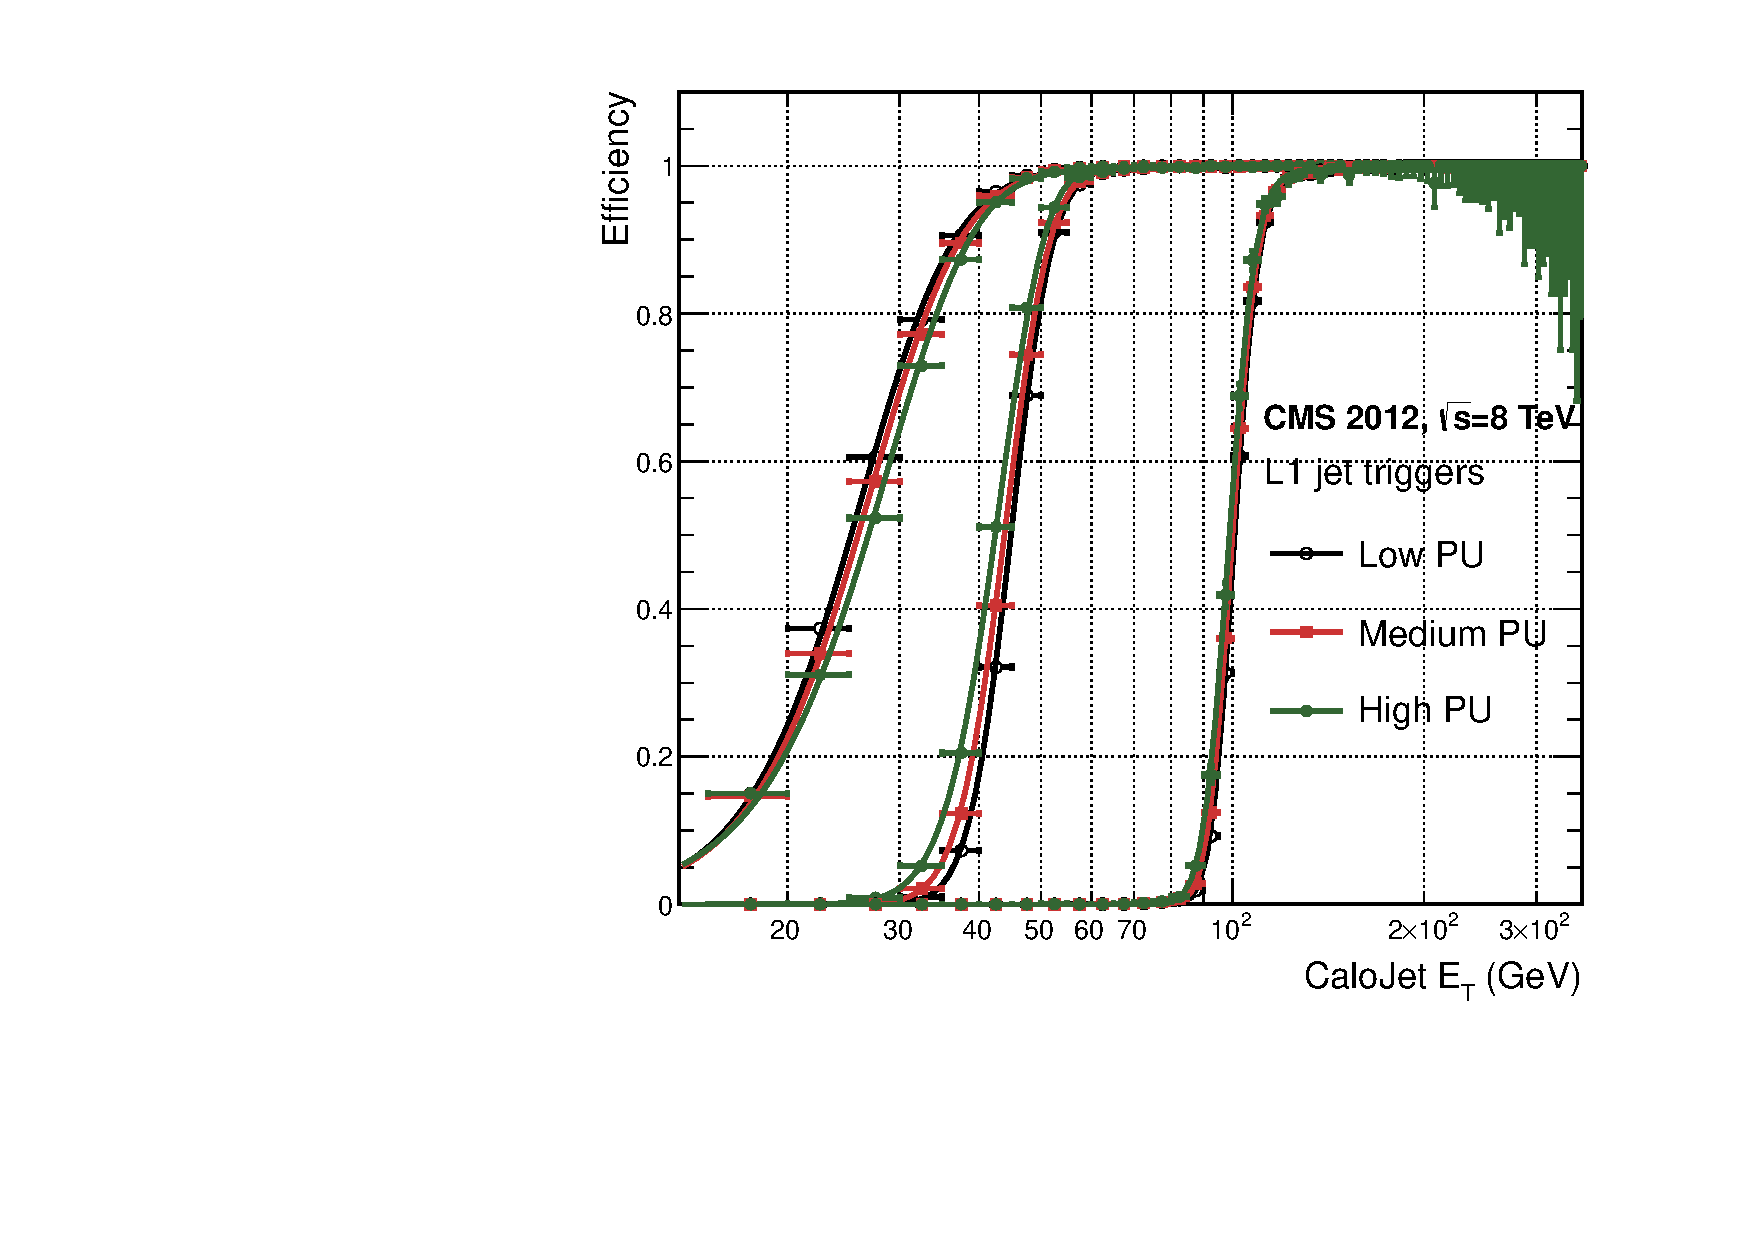
\includegraphics[width = 1.0\linewidth]{plots/jetpt_RunC_calopu.pdf}
\end{minipage}
\quad
\begin{minipage}[b]{0.46 \linewidth}
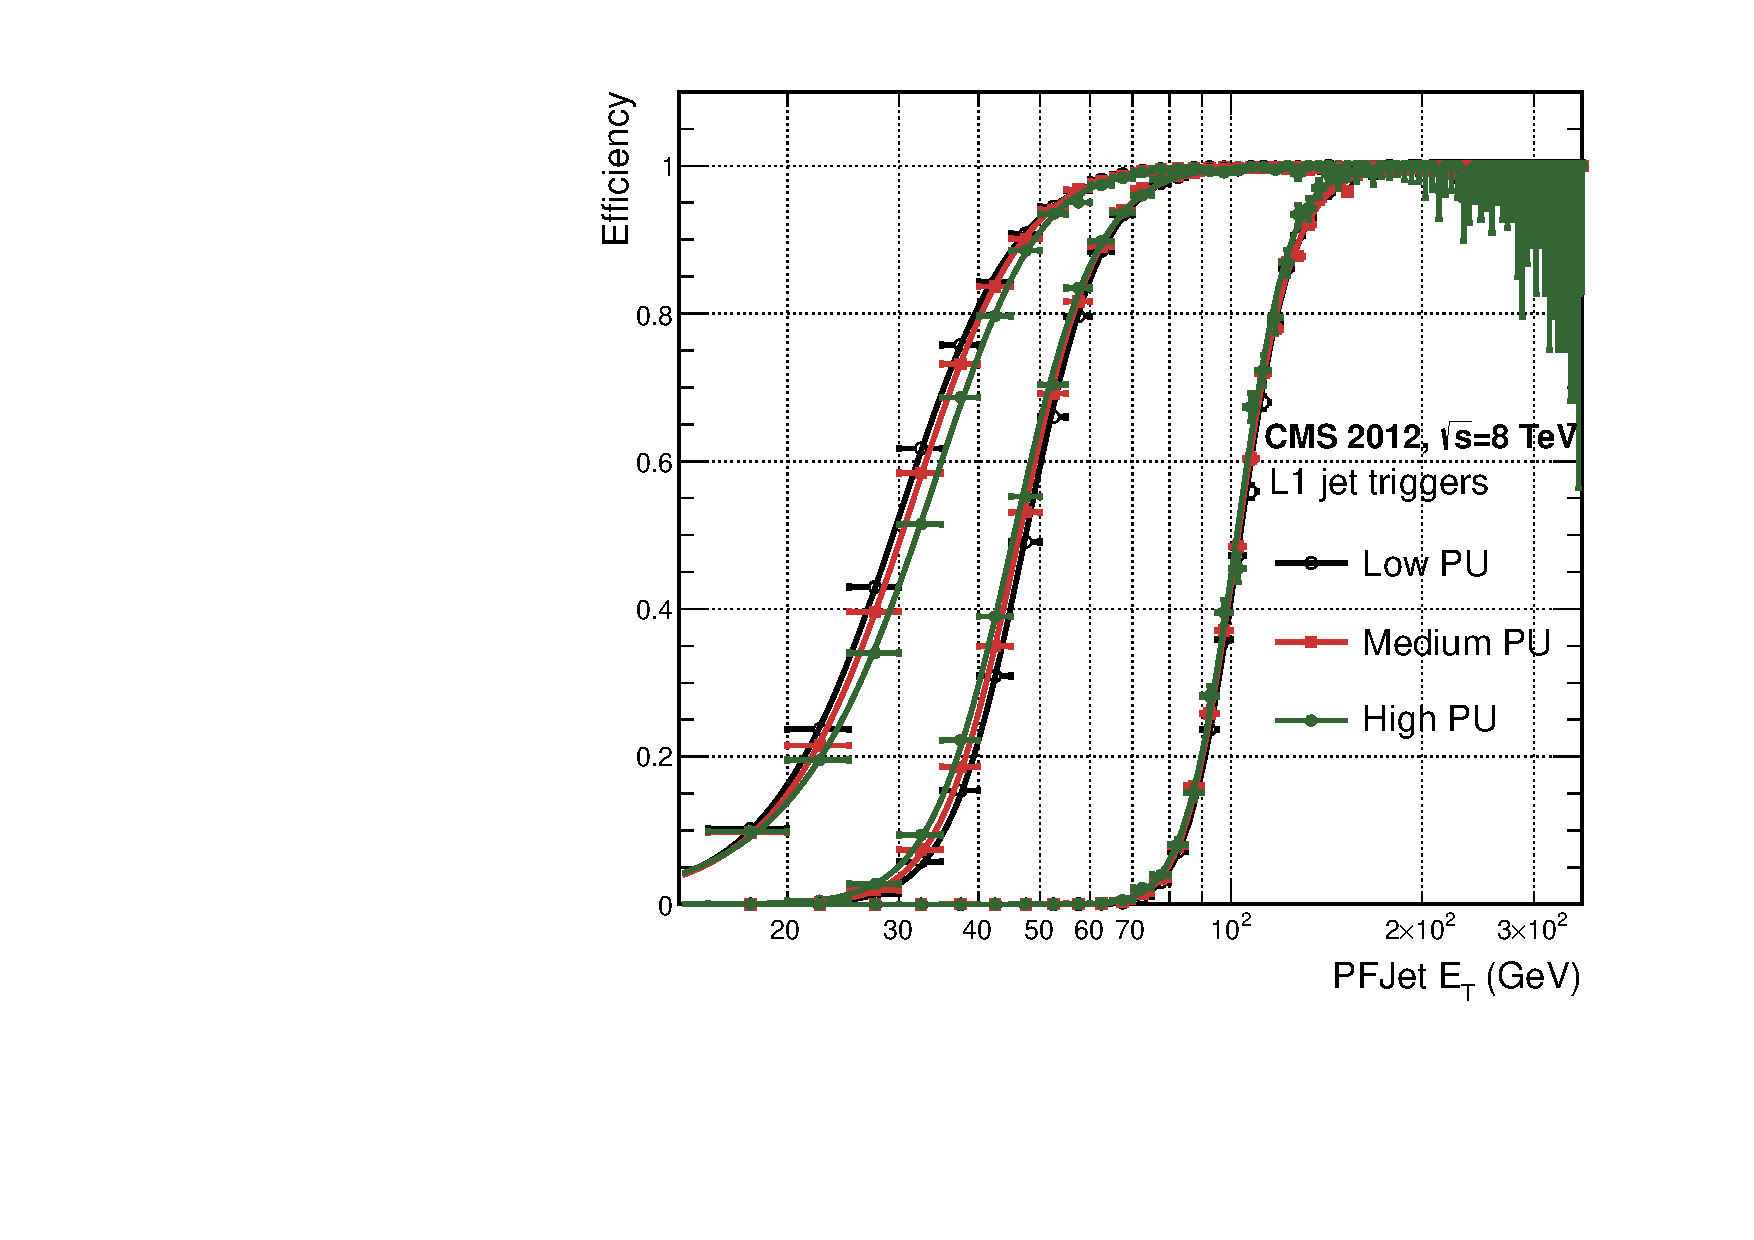
\includegraphics[width = 1.0\linewidth]{plots/jetpt_RunC_pfpu.pdf}
\end{minipage}
\quad
\caption[\L1 jet efficiency turn-on curves as a function of the leading offline $\et$ \Calo (left) and \PF (right) jet, for low, medium and high pile-up conditions.]{\L1 jet efficiency turn-on curves as a function of the leading offline $\et$\Calo (left) and \PF (right) jet, for low, medium and high pile-up conditions.}
\label{fig:l1jet-calopf-pu} 
\end{figure}



\begin{table}[ht]
%\begin{center}
\footnotesize
\begin{tabular*}{1.0\textwidth}{@{\extracolsep{\fill}}c|cc|cc|cc}
\hline
\multicolumn{1}{c}{Vertices} & \multicolumn{2}{c}{ 0-10 } & \multicolumn{2}{c}{11-20} & \multicolumn{2}{c}{$>$ 20}   \\ 
\multicolumn{1}{c}{} & $\mu$ & \multicolumn{1}{c}{$\sigma$} & $\mu$ & \multicolumn{1}{c}{$\sigma$} & $\mu$ & $\sigma$ \\ \hline\hline
\texttt{L1\_SingleJet16} & 19.9 $\pm$ 0.1 & 6.1 $\pm$ 0.3  & 20.8 $\pm$ 0.1 & 6.5 $\pm$ 0.1 & 22.3 $\pm$ 0.2 & 7.5 $\pm$ 0.1\\ 
\texttt{L1\_SingleJet36}& 41.8 $\pm$ 0.1 & 4.6 $\pm$ 0.1 & 40.9 $\pm$ 0.1 & 5.1 $\pm$ 0.1 & 40.6 $\pm$ 0.6 & 5.9 $\pm$ 0.2 \\ 
\texttt{L1\_SingleJet92} & 95.9 $\pm$ 0.2 & 5.4 $\pm$ 0.1 & 95.2 $\pm$ 0.2 & 5.6 $\pm$ 0.1 & 94.5 $\pm$ 0.6 & 6.2 $\pm$ 0.3  \\ 
\end{tabular*}
%\end{center}
\caption[Results of a cumulative \ac{EMG} function fit to the efficiency turn-on curves for \L1 single jet triggers in the 2012 run period C, for low,medium and high pile-up conditions.]{Results of a cumulative \ac{EMG} function fit to the efficiency turn-on curves for \L1 single jet triggers in the 2012 run period C,  measured from isolated $\mu$ triggered data. The turn-on point, $\mu$, and resolution, $\sigma$, of the \L1 jet triggers are measured with respect to offline \Calo jets in low (left), medium (middle) and high (right) pile-up conditions. }
\label{tab:l1jcaloputable}
\end{table}

\begin{table}[ht]
%\begin{center}
\footnotesize
\begin{tabular*}{1.0\textwidth}{@{\extracolsep{\fill}}c|cc|cc|cc}
\hline
 \multicolumn{1}{c}{Vertices} & \multicolumn{2}{c}{ 0-10 } & \multicolumn{2}{c}{11-20} & \multicolumn{2}{c}{$>$ 20}   \\ 
 \multicolumn{1}{c}{} & $\mu$ & \multicolumn{1}{c}{$\sigma$} & $\mu$ & \multicolumn{1}{c}{$\sigma$} & $\mu$ & $\sigma$ \\ \hline\hline
\texttt{L1\_SingleJet16} & 21.1 $\pm$ 0.1 & 7.16 $\pm$ 0.05 & 22.34 $\pm$ 0.1 & 7.9 $\pm$ 0.1 & 24.6 $\pm$ 0.2 & 9.5 $\pm$ 0.1 \\ 
\texttt{L1\_SingleJet36} & 39.6 $\pm$ 0.1 & 7.4 $\pm$ 0.1 & 38.4 $\pm$ 0.1  & 7.4 $\pm$ 0.1 & 37.1 $\pm$ 0.2 & 7.5 $\pm$ 0.1 \\ 
\texttt{L1\_SingleJet92} & 91.6 $\pm$ 0.3 & 11.3 $\pm$ 0.2 & 91.4 $\pm$ 0.3 & 11.2 $\pm$ 0.1 & 90.0 $\pm$ 0.9 & 12.1 $\pm$ 0.4  \\ 
\end{tabular*}
%\end{center}
\caption[Results of a cumulative \ac{EMG} function fit to the efficiency   turn-on curves for Level-1 single jet triggers in the 2012 run period C, for low,medium and high pile-up conditions.]{Results of a cumulative \ac{EMG} function fit to the efficiency   turn-on curves for Level-1 single jet triggers in the 2012 run period C, measured from isolated $\mu$ triggered data. The turn-on point, $\mu$, and resolution, $\sigma$, of the \L1 jet triggers are measured with respect to offline \PF jets in low (left), medium (middle) and high (right) pile-up conditions. }
\label{tab:l1pfputable}
\end{table}

No significant drop in efficiency is observed in the presence of a high number of primary vertices. The increase in hadronic activity in higher pile-up conditions, combined with the absence of pile-up subtraction for L1 jets (compared to reconstructed jets, see Section (\ref{subsec:cmsobjects-jets})), results in the expected observation of a decrease in the $\mu$ value of the efficiency turn-ons as a function of pile-up. Similarly, the resolution, $\sigma$, of the turn-ons are found to worsen at a higher number of primary vertices due to the increasing size of the pile-up corrections being applied to the offline reconstructed jets. 

These features are further emphasised when a direct comparison of \L1 and offline lead jet quantities is made in events in which the lead reconstructed jet in the event has been matched to a \L1 jet. This can be shown via the variable

\begin{equation}
\Delta  E_{\text{L1-Offline}} = \frac{(\text{L1 E}_{T} -  \text{Offline E}_{T})}{\text{Offline E}_{T}}
\label{eq:jetresolution}
\end{equation}

in bins of matched leading offline jet $\et$. The results of these individual fits categorised as a function of matched leading offline jet $\et$ can be found in Appendix (\ref{app:jetpuresolution}), where each of the distributions are fitted with an \ac{EMG} function as defined in Equation (\ref{eq:emg}).

The $\mu$, $\sigma$ and $\lambda$ values extracted for the low, medium and high pile-up conditions are shown for Calo and PF jets in Figure \ref{fig:jetptresultspu} and Figure \ref{fig:pfjetptresultspu} respectively with no \L1 trigger requirements made. The central value of $\Delta  E_{\text{L1-Offline}}$ is observed as expected, to increase as a function of jet $\et$, whilst the resolution also improves as a function of increasing offline jet $\et$ for all pile-up categories. 

When comparisons are made between the individual pile-up scenarios, it can be seen that in the presence of higher pile-up , $\mu$ is seen to shift to larger values and a poorer resolution, $\sigma$, observed. This is particularly evident at low lead jet transverse energy values where additional energy from isotropic deposits lead to a smaller difference between \L1 and offline jet energies at higher pile-up. These differences between the different pile-up scenarios are seen to increase with each successive pile-up category, and can once again be attributed to an increasing number of soft pile-up jets that add to the transverse energy of the lead jet from the primary interaction. 

However, when comparisons of the trigger performance at larger lead jet transverse energy values ($>100$ \GeV) are made, similar performance is observed between the separate pile-up categories.


\begin{figure}[h!]
  \vspace{20pt}
	\centering
	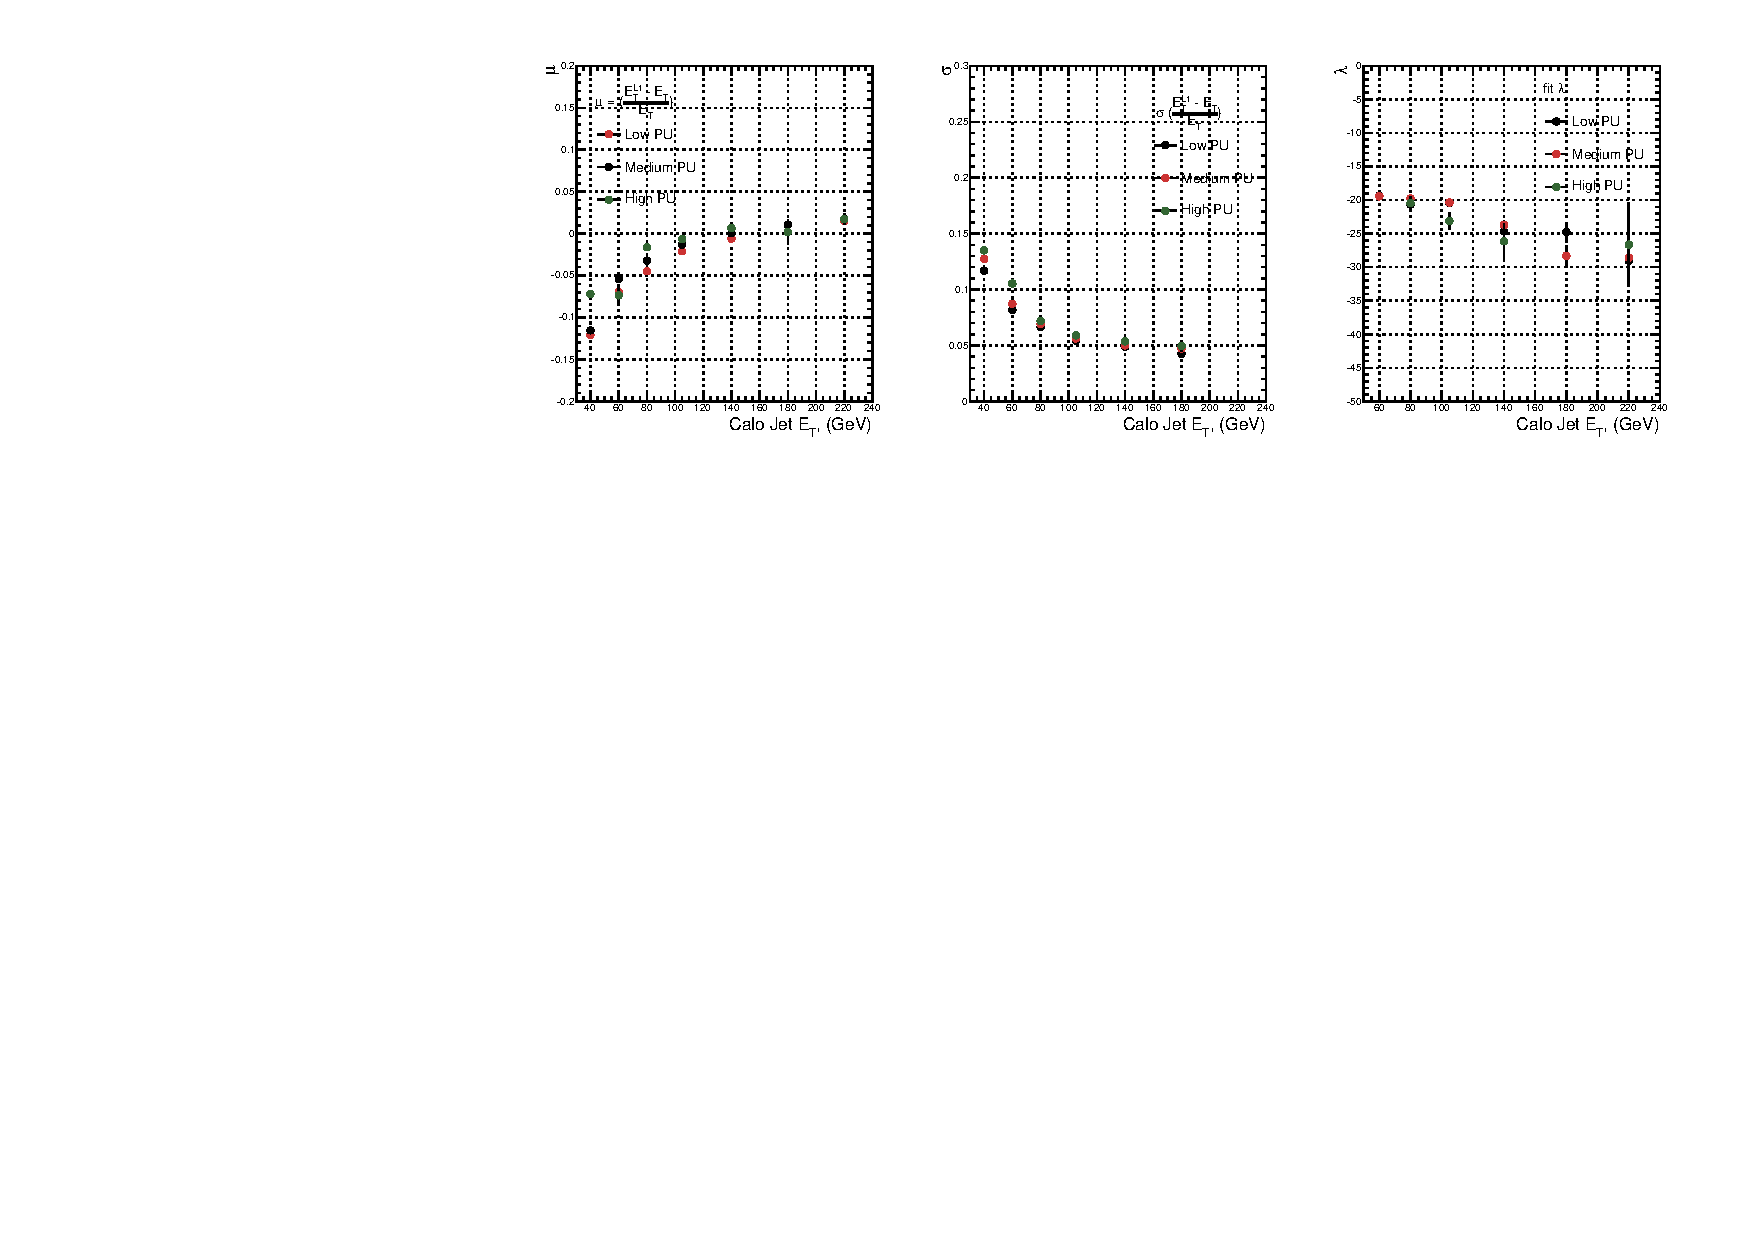
\includegraphics[width=0.7\textwidth]{plots/res_CaloJet_summary.pdf}
	\caption[Fit values from an \ac{EMG} function fitted to the resolution plots of leading Calo jet $\et$ measured as a function of  $\Delta  E_{\text{L1-Offline}}$  for low, medium and high pile-up conditions. ]{Fit values from an \ac{EMG} function fitted to the resolution plots of leading Calo jet $\et$ measured as a function of  $\Delta  E_{\text{L1-Offline}}$  for low, medium and high pile-up conditions. The plots show the mean $\mu$ (left) and resolution $\sigma$ (righ) of the Gaussian term.}
	\label{fig:jetptresultspu}
\end{figure}

\begin{figure}[h!]
  \vspace{20pt}
        \centering
        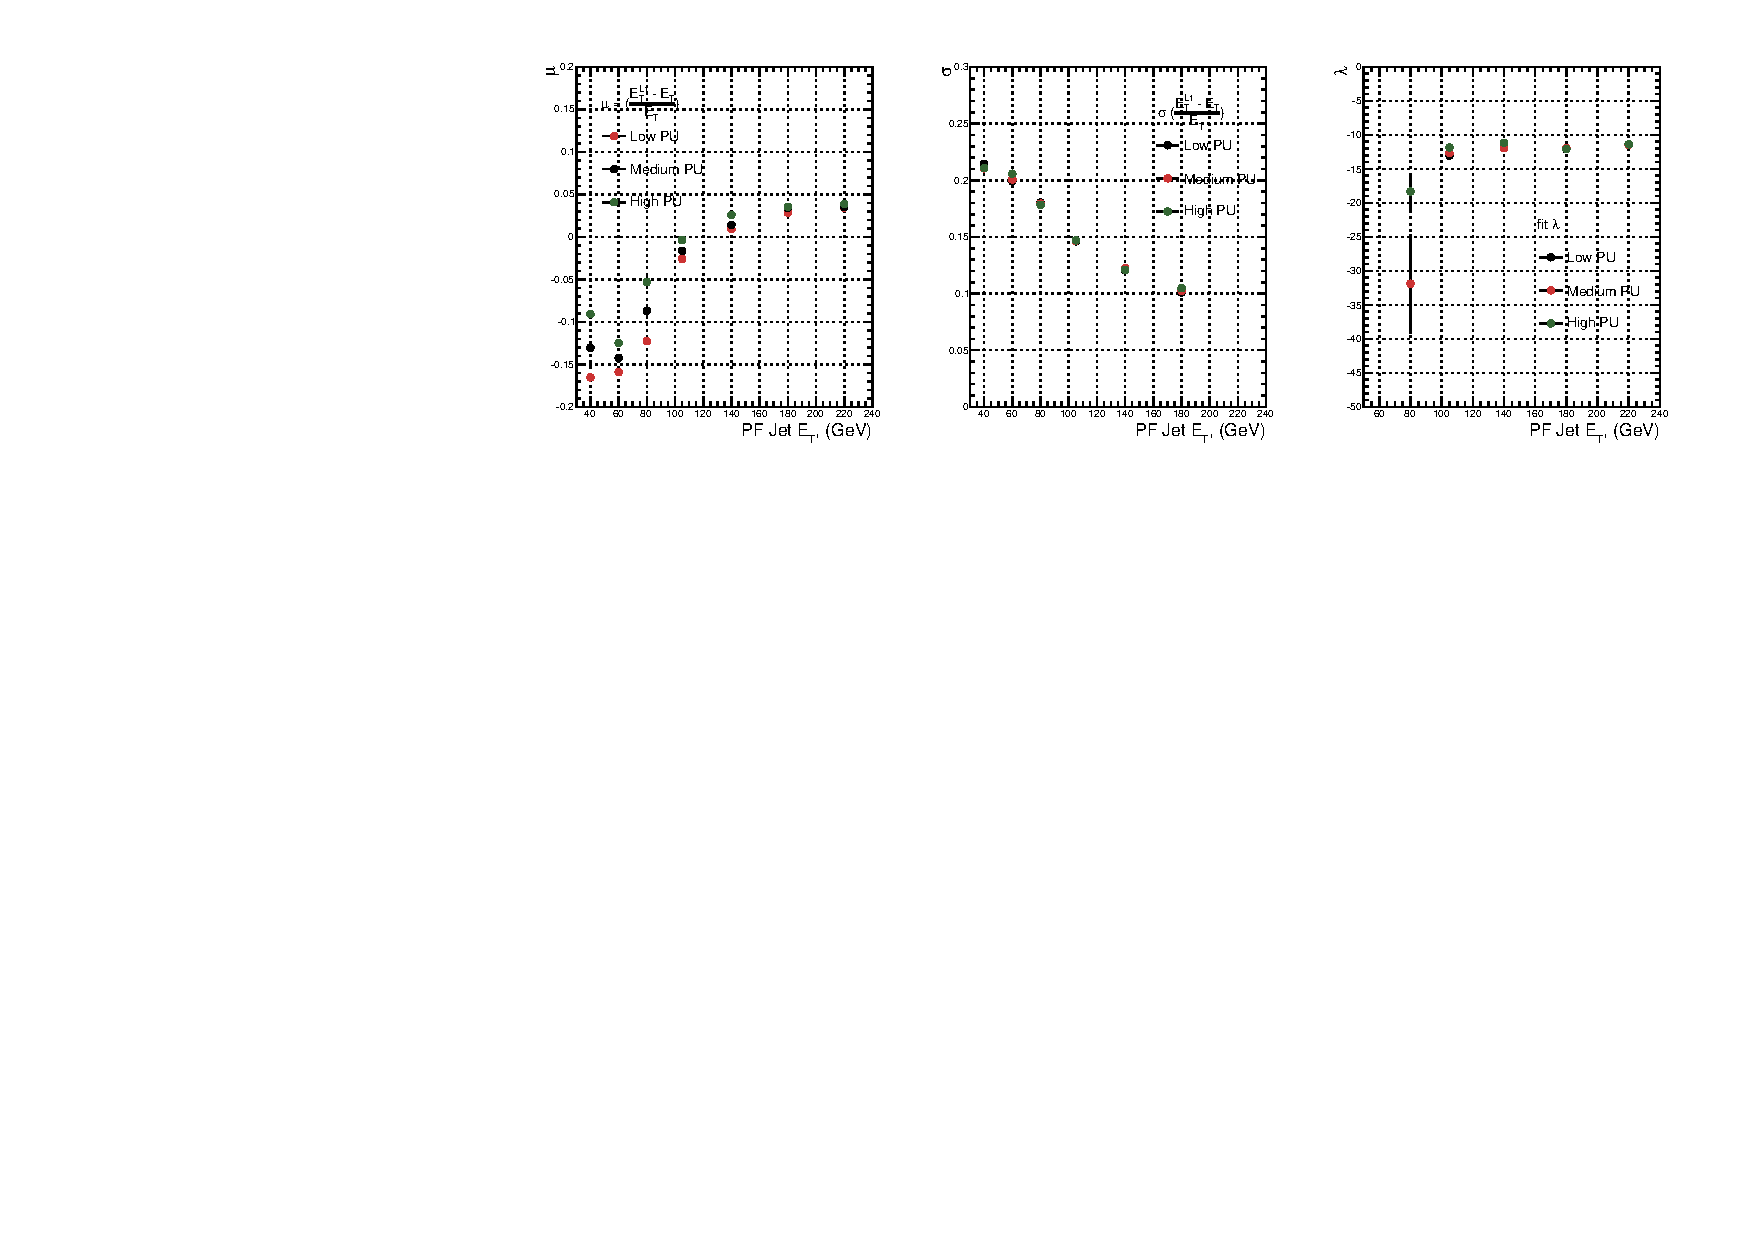
\includegraphics[width=0.7\textwidth]{plots/res_PFJet_summary.pdf}
        \caption[Fit values from an \ac{EMG} function fitted to the resolution plots of leading PF jet $\et$ measured as a function of $\Delta  E_{\text{L1-Offline}}$  for low, medium and high pile-up conditions.]{Fit values from an \ac{EMG} function fitted to the resolution plots of leading PF jet $\et$ measured as a function of  $\Delta  E_{\text{L1-Offline}}$  for low and medium pile-up conditions. The plots show the mean $\mu$ (left) and resolution $\sigma$ (right) of the Gaussian term.}
        \label{fig:pfjetptresultspu}
\end{figure}

The resolution of the \L1 jet based energy sum quantities, $\mht$ and $\theht$ parameterised as in Equation (\ref{eq:jetresolution}), can be found in Appendix (\ref{app:jetenergysums}).

\section{Summary}
\label{subsec:l1summary}

The performance of the \CMS Level-1 Trigger has been studied and evaluated for jets and jet energy sum quantities using data collected during the 2012 \ac{lhc} 8 TeV run. These studies include the effect of the introduction of a 5 \GeV jet seed threshold into the jet clustering algorithm. The purpose of this change was to mitigate the increase in \L1 trigger cross-sections, due to larger isotropic energy deposits from an increased number of secondary interactions, whilst not adversely affecting the efficiency of these triggers. Measurements are made for a range of \L1 jet quantities and thresholds, where no significant change is observed in the measured efficiencies that would indicate a noticeable effect on the overall triggering performance of the detector. 